%%%%%%%%%%%%%%%%%%%%%%%%%%%%%%%%%%%%%%%%%%%%%%%%%%%%%%%%%%%%%%%%%%%%%%
%% ANONYMISED VERSION for double-blind peer review
%% Torddis manuscript adapted to Education and Information Technologies
%% Springer Nature LaTeX template v3.1 (December 2024), APA reference style
%% Journal: Education and Information Technologies (EAIT)
%% ISSN: 1360-2357 (print), 1573-7608 (online)
%%%%%%%%%%%%%%%%%%%%%%%%%%%%%%%%%%%%%%%%%%%%%%%%%%%%%%%%%%%%%%%%%%%%%%

\documentclass[pdflatex,sn-apa]{sn-jnl}% APA Reference Style (EAIT uses APA 7)

%%%% Standard Packages
\usepackage[T1]{fontenc}%
\usepackage[utf8]{inputenc}%
\usepackage{graphicx}%
\usepackage{multirow}%
\usepackage{amsmath,amssymb,amsfonts}%
\usepackage{amsthm}%
\usepackage{mathrsfs}%
\usepackage[title]{appendix}%
\usepackage{xcolor}%
\usepackage{textcomp}%
\usepackage{manyfoot}%
\usepackage{booktabs}%
\usepackage{algorithm}%
\usepackage{algorithmicx}%
\usepackage{algpseudocode}%
\usepackage{listings}%
\usepackage{tabularx}%
\usepackage{pgfplots}%
\usepackage{tikz}%
\usepackage{subcaption}%
\usepackage[export]{adjustbox}%
\usepackage{url}%

\pgfplotsset{compat=1.18}%
\graphicspath{{figs/}}%

%% Local helper macros used in the tables of the original manuscript
\newcommand{\datacell}[2]{\makebox[\linewidth][r]{#1\hspace{#2}}}%
\pgfmathsetmacro{\average}{81.46}%
\pgfmathsetmacro{\stdev}{11.65}%
\pgfmathsetmacro{\upperlimit}{\average+\stdev}%
\pgfmathsetmacro{\lowerlimit}{\average-\stdev}%

\raggedbottom%

\begin{document}

\title[Torddis for at-home learning]{Torddis: A Real-Time IoT and AI-Based System to Support At-Home Learning and Mitigate Parental Absenteeism}

%%=============================================================%%
%% Author identification suppressed for double-blind review.
%% The full author, affiliation, corresponding author, ORCID and
%% acknowledgement information is provided in a separate title page
%% uploaded to the editorial system.
%%=============================================================%%

\author*[1]{\fnm{Author} \sur{Anonymised}}\email{anonymised@example.org}

\affil*[1]{\orgname{Author affiliation anonymised for double-blind review}}

%%==================================%%
%% Unstructured abstract (150-250 words as per EAIT guidelines)
%%==================================%%

\abstract{
    Parental absenteeism during out-of-school study hours has intensified in recent years, undermining the academic performance and self-regulation of primary school children. This paper introduces Torddis, a real-time system that combines Internet of Things (IoT) hardware and Artificial Intelligence (AI) models to support at-home learning when tutors cannot provide continuous supervision. Torddis integrates an ESP32-CAM/NodeMCU device with a mobile application; it detects facial expressions indicative of inattention, unauthorised objects on the desk, and signs of drowsiness, and returns visual and auditory alerts that promote self-correction. The system was designed and validated following the Test-Driven Development Methodology for IoT Systems (TDDM4IoTS). A pilot deployment was carried out in twelve families over one week; tutors evaluated the prototype through the System Usability Scale (SUS) and a purpose-built seven-item Likert questionnaire on perceived effectiveness. Torddis obtained a mean SUS score of 81.46\% (SD = 11.65), corresponding to a ``Good'' usability level. Statistical analyses (Shapiro--Wilk, ANOVA, Kruskal--Wallis, Pearson and Spearman correlations) revealed a strong positive association between the use of the device and tutor-perceived improvements in children's concentration and self-regulation. The findings support the pedagogical value of AI-enabled IoT tools for autonomous learning at home and outline avenues for larger and longer-term evaluations.
}

\keywords{Educational technology, Internet of Things, Artificial intelligence, Self-regulated learning, Home-based learning, Usability evaluation}

\maketitle

%%=========================================================================%%
%% Body of the manuscript (identical to the full version, with all
%% author-identifying references replaced or removed in the body itself).
%%=========================================================================%%

	\section{Introduction}
	\label{section:first}
		Over the last decade, accelerated lifestyles and increasing workloads have contributed to a rise in parental absenteeism during the hours designated for schoolwork at home, particularly among primary school students. This situation has underscored the need for technological solutions to compensate for the lack of supervision \citep{Seidu2022Truancy,Ketsman2025Mapping}.
		
		The absence of parental support directly impacts the academic performance of young learners. Teachers have observed a decline in indicators related to performance and discipline, which may adversely affect students’ self-esteem and other psychosocial dimensions. Furthermore, the literature emphasizes that emotional support in the home is a fundamental pillar for maintaining children’s focus on their studies \citep{Seidu2022Truancy}.
		
		Emotional interference not only influences educational outcomes but also significantly affects other aspects of students’ lives \citep{Ake2023}. In this context, a family environment that fosters positive communication and genuine interaction can enhance students’ well-being and social skills \citep{Navarro2024}. However, to effectively address the challenges associated with attention and emotional regulation, it is crucial to incorporate technological tools that integrate Artificial Intelligence (AI) and the Internet of Things (IoT). These technologies enable the monitoring and measurement of children's distractions, providing essential data to support decision-making processes aimed at improving attention and learning outcomes \citep{Alvear-Puertas2017,Berrezueta-Guzman2021}.
		
		The use of AI- and IoT-based technologies not only contributes to the improvement of academic performance but also promotes self-regulation skills in students, which are essential for their cognitive and socio-emotional development \citep{Mohamed2018Implementing}. The feedback provided by such technologies helps students identify their distractions and take corrective actions, strengthening their ability to manage time and concentrate on academic tasks. Consequently, technological tools emerge as valuable resources to complement the positive influence of the family environment and to foster self-regulated learning, creating a comprehensive approach that encompasses both educational and personal development \citep{Thinyane2016AUG}.
		
		Students' ability to concentrate is a crucial factor in their capacity to learn and apply knowledge delivered by educators. In a study conducted by \cite{Terraza2022}, a system was proposed to monitor students’ attention in an online learning environment using computer vision algorithms. The authors implemented a Recurrent Neural Network (RNN) to identify facial landmarks, detecting whether a student maintained a frontal position toward the device used to attend virtual classes. Their study reveals some limitations present in current proposals.
		
		On the other hand, the work of \cite{Berrezueta-Guzman2021} introduced a robotic system designed to interact with children diagnosed with Attention Deficit Hyperactivity Disorder (ADHD), helping them correct unhealthy habits and inappropriate behaviors associated with this condition. Although effective within its specific scope, this system is exclusively oriented toward children with ADHD. Its generalized application may lead to disruptions for children without this condition, and it lacks notification, alert, or alarm functionalities to inform tutors about potential incidents.
		
		To promote active tutor participation and enhance children’s emotional well-being, this paper introduces Torddis\footnote{From Latin \textit{\textbf{Tor}queo \textbf{d}iscerno \textbf{dis}cipulus}, meaning ``detection of deviation or change in the student’s attention.''}, a technological solution designed to monitor student behavior while they autonomously perform academic tasks at home, notifying tutors of any significant event and conveying to students the feeling that they are not alone. In addition, Torddis is capable of playing sounds, including personalized messages according to user preferences.
		
		To achieve these objectives, Torddis employs advanced computer vision algorithms and deep learning techniques. The system includes a mobile application for tutors and an IoT device that analyzes children's behavior while they complete schoolwork independently. Developed following the TDDM4IoTS methodology [reference anonymised], Torddis features a holistic approach, enabling tutors to monitor and respond in real time to signs of inattention. Key functionalities include the detection of facial expressions associated with core emotions, identification of drowsiness, and recognition of inappropriate use of distractive objects during academic activities. These features allow tutors to encourage their children to remain focused through the use of visual and auditory reinforcement cues \citep{Al-Gburi2023,Enadula2021,Terraza2022}.
		
		Torddis is designed to strengthen metacognitive skills such as time management and sustained attention, which are essential components of modern autonomous learning. Its emphasis on proactive supervision addresses the need to support children during a critical stage of development, providing tutors with a valuable tool that complements traditional supervision at home and contributes to improving educational outcomes within this population.
		
		This article is organised as follows: Section~\ref{section:third} presents a review of the most relevant related work published in the last ten years. Section~\ref{section:fourth} describes the design and development of the Torddis system, including the applied methodology, the hardware and software artefacts and the AI models used. Section~\ref{section:fifth} outlines the methodological design of the pilot study and its experimental validation. Section~\ref{section:sixth} reports the empirical results, including the usability evaluation, the recognition performance and the statistical analysis of the guardians' responses. Section~\ref{section:discussion} discusses the main findings and their pedagogical implications, and Section~\ref{section:eight} concludes the article and suggests avenues for future research.
				
	\subsection{Theoretical Background}
\label{sec:theoretical-background}
    Torddis is grounded in the paradigm of self-regulated learning \citep{Zimmerman2000Attaining, Panadero2017Review}, which describes how learners plan, monitor and adjust their behaviour to attain academic goals. When adult supervision is unavailable at home, self-regulation is precisely the skill children of primary school age are still developing. Recent evidence shows that AI-mediated feedback loops can scaffold this process by delivering timely, personalised cues that steer attention back to task \citep{Wang2025Development, Li2024Systematic}, and that Internet of Things (IoT) devices are especially well suited to unstructured domestic settings because of their unobtrusive form factor \citep{Ackermans2025Young}. Torddis integrates these two threads: it uses AI models to detect emotional, cognitive and contextual signs of distraction, and it uses IoT hardware to deliver personalised alerts in real time. In doing so, it acts as a mediator between student autonomy and external guidance, supporting the development of digital competence and academic self-management \citep{Loh2025Plugging, Mohamed2018Implementing, Echeverria2011AFramework}.

\section{Related Works}
	\label{section:third}
		The literature on the use of technologies for detecting and correcting student distractions is limited, particularly regarding the integration of IoT technologies for pedagogical purposes. Previous studies have addressed technological applications in child monitoring, yet few have explored how these technologies can be used to provide immediate feedback that promotes learning self-regulation and enhances educational outcomes in non-formal contexts. The state-of-the-art review process was conducted in accordance with the guidelines established by \cite{Kitchenham2007Guidelines}, whose methodology is presented in the diagram in Figure~\ref{fig:LRS}.
			
		\begin{figure}[!htbp]
			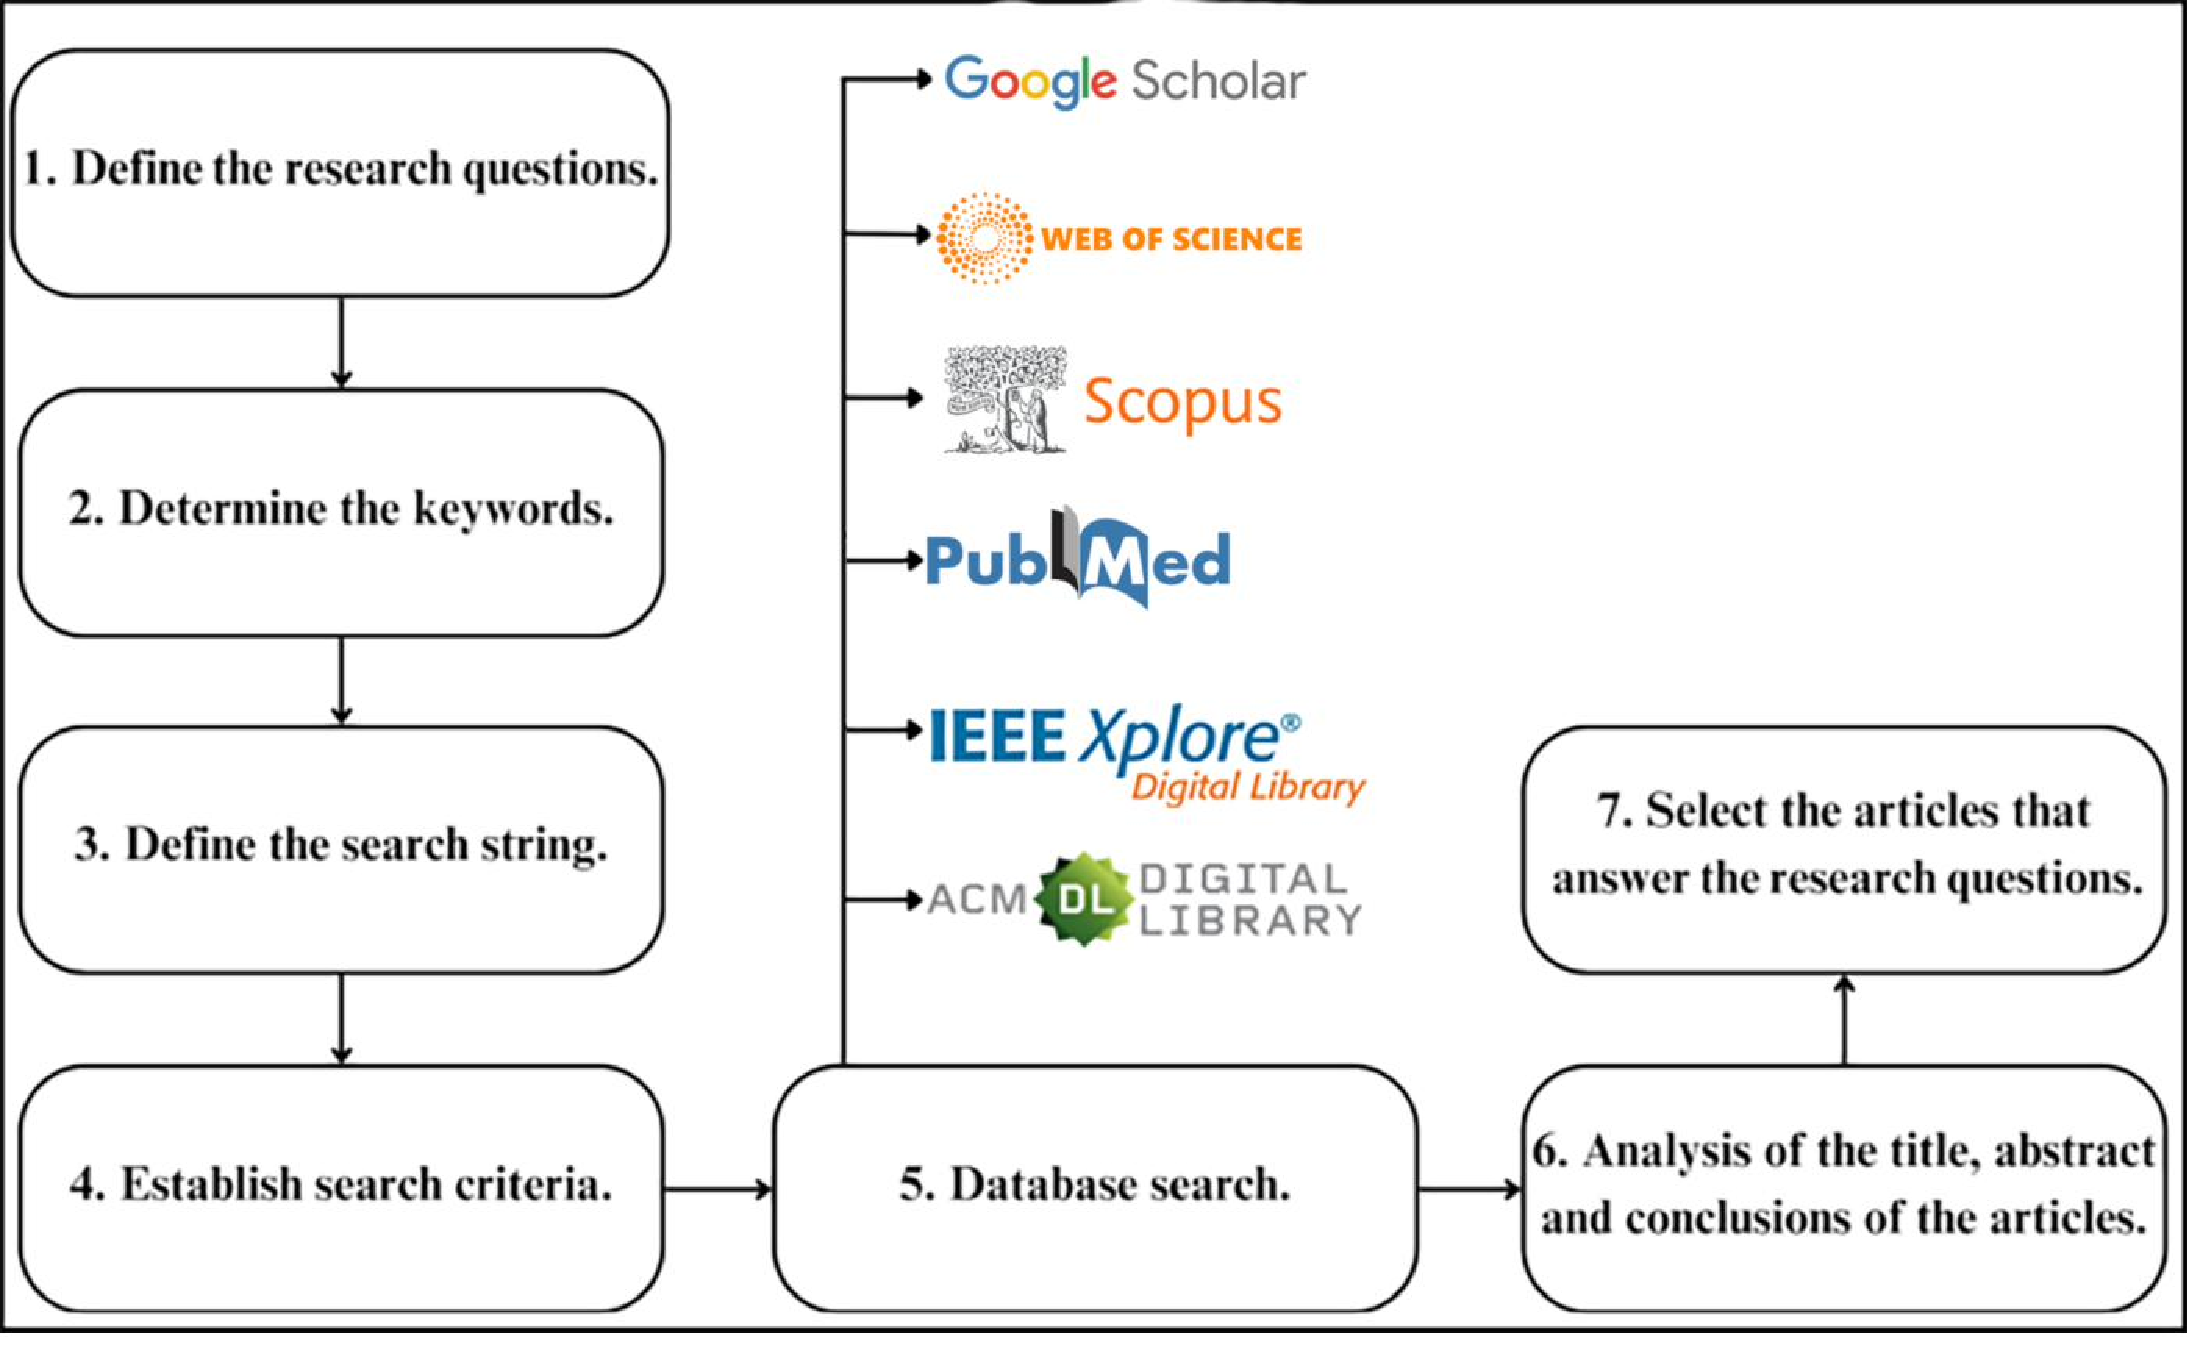
\includegraphics[width=\textwidth]{Figure_1}
			\caption{Literature review scheme.}
			\label{fig:LRS}
		\end{figure}   

		\subsection{Research Questions}
			This article addresses the critical issue of detecting student distractions during autonomous schoolwork. With the increasing availability of digital tools for education and the growing need for effective learning strategies, understanding how distractions impact student performance has become essential. The following research questions guide this comprehensive review of related works and inform the development of technological solutions aimed at improving children’s concentration and educational outcomes:
			
			\begin{itemize}
				\item \textit{RQ1:} Which AI and IoT technologies are most suitable for designing a system capable of monitoring children’s distractions during their school activities at home?
				
				\item \textit{RQ2:} What internal and external parameters can be used to detect distractions in children, and how should these be integrated into an IoT system to ensure effectiveness and personalization?
				
				\item \textit{RQ3:} How can a real-time IoT system foster key skills such as self-regulation, autonomous learning, and concentration in students working on school tasks at home?
				
				\item \textit{RQ4:} What are parents’ or tutors’ perceptions regarding the usefulness, usability, and effectiveness of an IoT system designed to support home learning, and how does this perception influence its acceptance?
			\end{itemize}
					
		\subsection{Search Strategy}
			Once the research questions were defined, relevant keywords were selected to retrieve the most recent publications from major scientific databases in this research field. These keywords were used to construct the search string, which was then adapted to the specific requirements of each selected database. The final search string was: (distraction OR distractions) AND (child OR children OR student) AND (homework OR ``school assignments'' OR ``school tasks'') AND (''object recognition´´ OR ``facial recognition'' OR ``gesture recognition'').
			
			The literature searches were conducted in high-prestige scientific databases, including ACM Digital Library, IEEE Xplore, PubMed, Scopus, and Web of Science. Additionally, Google Scholar was used to expand the search results and minimize the likelihood of omitting relevant studies related to our research. These platforms facilitated the identification of pertinent literature using predefined criteria.
			
			The selected documents came from recognized academic publishers such as ACM, Elsevier, Springer, IEEE, among others, ensuring the scientific quality and validity of the material analyzed. Table~\ref{tab:Results} presents the results of the initial search in these databases and in Google Scholar. The \textit{Duplicates} column shows the number of documents that had already been retrieved from other databases and were therefore excluded. After analyzing the title and abstract, a full-text review of the documents was conducted to determine whether they addressed any of the study's research questions. As a result of this final review, the total number of documents included in the analysis is shown in the \textit{Final Results} column of Table~\ref{tab:Results}.
			
			\begin{table}[!htbp]
				\caption{Results of the related works search.\label{tab:Results}}
				\centering
				\begin{tabular*}{\linewidth}{@{\extracolsep{\fill}}
						>{\raggedright\arraybackslash}p{3cm}
						>{\raggedleft\arraybackslash}p{2cm}<{\hspace*{8pt}}
						>{\raggedleft\arraybackslash}p{1.6cm}<{\hspace*{8pt}}
						>{\raggedleft\arraybackslash}p{2.4cm}<{\hspace*{8pt}}
						>{\raggedleft\arraybackslash}p{1.8cm}<{\hspace*{8pt}}
						@{}}
					\toprule
					\multicolumn{1}{c}{\textbf{\shortstack{Database/Search\\Engine}}} &
					\multicolumn{1}{c}{\textbf{\shortstack{Preliminary\\Results}}} &
					\multicolumn{1}{c}{\textbf{Duplicates}} &
					\multicolumn{1}{c}{\textbf{\shortstack{Title and Abstract\\Review}}} &
					\multicolumn{1}{c}{\textbf{\shortstack{Final\\Results}}} \\
					\midrule
					ACM             & 1       & 0  & 1  & 1  \\
					IEEE Xplore     & 3       & 0  & 2  & 2  \\
					PubMed          & 2       & 1  & 0  & 0  \\
					Scopus          & 22      & 3  & 19 & 15 \\
					Web of Science  & 8       & 6  & 2  & 2  \\
					Google Scholar  & 15\,400 & 19 & 16 & 6  \\
					\bottomrule
				\end{tabular*}
			\end{table}
						
		\subsection{Literature Analysis}
			In the scientific literature on technologies applied to the fields of education and child care, several approaches focus on the use of Artificial Intelligence (AI), the Internet of Things (IoT), and computer vision techniques to enhance learning and behavioral monitoring. Additionally, other studies have integrated these technologies to facilitate learning self-regulation, improve concentration, and foster academic engagement across different student populations.
			
		\subsubsection{Behavior Monitoring}
			Studies such as those by \cite{Akter2021}, \cite{Albrecht2014}, \cite{Berrezueta-Guzman2021}, \cite{Pelc2006}, \cite{VilliersRader2021}, \cite{Warren2015Brief}, and \cite{Washington2016AWereable} explore applications ranging from early diagnosis of Autism Spectrum Disorder (ASD) to improving emotion recognition in children with Attention Deficit Hyperactivity Disorder (ADHD). These studies employ advanced technologies such as AI and connected devices to analyze and respond to specific child behaviors in both controlled and everyday environments.
			
			For example, \cite{Akter2021} apply transfer learning\footnote{\textit{Transfer learning \cite{Akter2021}} refers to the extent to which learners can effectively and consistently apply the knowledge, skills, and attitudes acquired during a training activity to different contexts beyond the original learning environment. In essence, it assesses whether an educational experience promotes learning that can be generalized and sustained in real-life situations.} for ASD diagnosis through facial recognition. Similarly, \cite{Pelc2006} focus on recognizing emotions in children with ADHD using validated photographs, while \cite{Albrecht2014} investigate visual search strategies in children with ASD. \cite{Berrezueta-Guzman2021} evaluate the use of a robotic assistant to support academic tasks for children with ADHD, and \cite{VilliersRader2021} examine how gestures can direct attention toward word-object relationships in children with ASD.
			
			Other studies, such as \cite{Boumiza2017}, \cite{DaCosta2023}, \cite{Enadula2021}, \cite{Farsani2020}, \cite{Hachad2020}, \cite{James2019}, \cite{Kulkarni2023}, \cite{Kumar2024Zoom}, \cite{Muller2018ArchnSmile}, \cite{Narkhede2023}, and \cite{Ozdamli2022}, also address issues related to safety, engagement, and interaction through monitoring technologies. For instance, \cite{Hachad2020} and \cite{James2019} employ facial recognition to monitor student safety on school buses and attendance in classrooms, respectively. Likewise, \cite{Ozdamli2022} use computer vision technologies to recognize emotions and detect cheating during online exams.
			
			In addition, \cite{Campbell2015Using} and \cite{Ucar2022Recognizing} present systems designed to monitor distractions in real time. For example, \cite{Campbell2015Using} use multispectral imaging to detect distractions caused by mobile devices, while \cite{Ucar2022Recognizing} employ facial recognition and head pose estimation to assess student engagement in virtual classes. Other works such as \cite{Argel2023Intellitell}, [reference anonymised], and \cite{Nguyen2019} also focus on behavioral evaluation using advanced technologies like YOLOv3 for real-time monitoring and dynamic adjustment of teaching strategies.
			
			Finally, studies such as \cite{Boumiza2017} and \cite{DaCosta2023} explore monitoring in contexts such as automated tutoring systems and school transportation within smart cities, highlighting the use of facial recognition to personalize educational experiences and enhance safety.
			
		\subsubsection{Technology for Autonomous Learning}
			Other studies focus on promoting self-regulation, concentration, and academic engagement by integrating technologies that support autonomous learning in diverse contexts. For instance, \cite{Bembich2016Future} investigate the use of digital technologies for future educators, providing self-regulation strategies to manage distractions. Similarly, \cite{Peters2003Self} examine how hypertext environments can improve volitional control and distraction management in digital autonomous learning.
			
			\cite{Roberts2020Task} analyze how secondary students use digital records to self-regulate and reflect on their academic progress. On the other hand, \cite{Adcroft2018Developing} combine digital technologies with time management and mindfulness practices to help students improve their focus and self-regulation in daily tasks.
			
			Studies such as \cite{Salter2014Exploring} and \cite{Palmer2022impact} integrate technologies and platforms to monitor and assess self-regulation skills. While \cite{Salter2014Exploring} adopt a whole-school approach, \cite{Palmer2022impact} focus on synchronous hybrid teaching in a pharmacotherapy course.
			
			\cite{Muljana2022Instructional} and \cite{Wang2022Empowering} explore specific strategies to promote self-regulation. \cite{Muljana2022Instructional} analyze how instructional professionals use social media to develop self-directed learning, while \cite{Wang2022Empowering} investigate the reduction of digital distractions among university students through self-regulation skills.
			
			Additionally, \cite{Hartley2022Smartphone} and \cite{Labar2019Interplay} examine the impact of mobile device use on attention and multitasking. While \cite{Labar2019Interplay} take a psychological approach to analyze time perception, \cite{Hartley2022Smartphone} focus on how smartphone use directly affects self-regulation abilities.
			
			These studies reflect a diverse range of approaches to self-regulation and the improvement of autonomous learning, employing technological strategies to reduce distractions, enhance volitional control, and foster academic engagement.
			
		\subsubsection{Comparison of Torddis with Previous Works}
			The literature analysis reveals significant progress in the use of advanced technologies to address educational and child care challenges. However, Torddis stands out as a comprehensive solution that integrates IoT, computer vision, and AI to deliver adaptive and proactive supervision in various environments. The following comparison outlines how Torddis overcomes limitations identified in the reviewed references.
			
			In the domain of behavioral monitoring, works such as \cite{Akter2021}, \cite{Pelc2006}, and \cite{Albrecht2014} employ facial recognition and visual analysis for diagnosing ASD and ADHD. While these approaches are valuable for understanding behavioral patterns, they lack real-time intervention capabilities—something Torddis provides through proactive alerts that redirect students' attention. In contrast, studies like \cite{Campbell2015Using}, \cite{Ucar2022Recognizing}, and \cite{Argel2023Intellitell} focus on identifying distractions but do not include features for adapting to domestic environments, a less structured context that Torddis effectively addresses.
			
			Additionally, research by \cite{Berrezueta-Guzman2021}, \cite{VilliersRader2021}, and \cite{Washington2016AWereable} introduces wearable and robotic technologies for children with developmental disorders. While these proposals offer personalized classroom support, they do not extend to home settings or enable continuous monitoring without constant adult intervention. Meanwhile, \cite{Muller2018ArchnSmile} focuses on playful activities using facial recognition for entertainment, and \cite{Nguyen2019} employs posture and gesture recognition to assess student engagement in classrooms. In contrast, Torddis balances monitoring of school task performance with strategies to enhance attention.
			
			In terms of safety and educational personalization, studies such as \cite{Hachad2020}, \cite{James2019}, and \cite{Boumiza2017} apply facial recognition for administrative tasks such as attendance and school transportation safety. However, they do not address pedagogical integration or adaptive student behavior monitoring. Similarly, systems like those proposed by \cite{DaCosta2023}, \cite{Kumar2024Zoom}, and \cite{Narkhede2023} employ technologies to detect emotions and attention during academic activities, but they fail to integrate distractor detection and proactive responses as Torddis does.
			
			Regarding technologies for autonomous learning, studies such as \cite{Bembich2016Future}, \cite{Roberts2020Task}, and \cite{Peters2003Self} focus on promoting self-regulation through digital tools. \cite{Muljana2022Instructional} analyze how instructional designers use social media to support self-regulation, but these strategies depend entirely on user commitment and lack automated attention redirection capabilities. In contrast, \cite{Palmer2022impact}, \cite{Adcroft2018Developing}, and \cite{Salter2014Exploring} introduce pedagogical practices such as mindfulness and hybrid teaching but do not incorporate advanced technologies like those implemented in Torddis for direct learning process intervention.
			
			In the context of multitasking and digital distractions, studies such as \cite{Hartley2022Smartphone}, \cite{Labar2019Interplay}, and \cite{Farsani2020} examine the impact of mobile devices on attention and academic engagement. While these works identify key issues, Torddis surpasses them by automatically detecting device-generated distractions and applying immediate corrective strategies. Furthermore, studies like [reference anonymised] and \cite{Wang2022Empowering} address digital distractions from gestural and pedagogical perspectives, respectively, but do not offer real-time automated interventions.
			
			Finally, works such as \cite{Kulkarni2023}, \cite{Enadula2021}, \cite{Ozdamli2022}, and \cite{Warren2015Brief} highlight the use of advanced technologies for educational interaction and emotion detection. However, these studies do not consider the multidimensional approach that Torddis introduces by combining emotional, cognitive, and contextual analysis to intervene effectively in home environments during academic activities.
			
			In conclusion, while the reviewed studies offer meaningful advances in specific areas, Torddis emerges as an integrated solution that not only overcomes the technical limitations of existing systems but also addresses the dynamic needs of educational and child supervision environments with a proactive and adaptive approach.
	
	\section{Torddis Development}
	\label{section:fourth}
		The development of the Torddis system followed a structured methodology to ensure the effective integration of hardware and software components, aiming to provide a comprehensive tool for monitoring and improving students’ concentration at home.
		
		More specifically, Torddis was developed using the TDDM4IoTS methodology [reference anonymised]. This methodology is one of the most comprehensive in terms of the system lifecycle [reference anonymised], and has been validated and evaluated in various application domains  [reference anonymised]. During the development of the proposed system, all stages of the methodology were applied, except the final one—maintenance—due to the system’s short lifespan at the time of writing this article. Furthermore, this methodological framework facilitates early error detection, contributing to reduced costs and development time while enabling cleaner code \citep{Beck2002TDD}.
		
		The project team was composed of the authors of this work, with the roles of each member detailed in Table \ref{tab:Roles}.
		
		\begin{table}[!htbp]
			\caption{Roles performed by team members.\label{tab:Roles}}
			\centering
			\begin{tabularx}{0.8\textwidth}{>{\raggedright\arraybackslash}X >{\raggedright\arraybackslash}X}
				\toprule
				\multicolumn{1}{c}{\textbf{Role}} & \multicolumn{1}{c}{\textbf{Member}} \\
				\midrule
				Client/End User & Author 5, Author 6, and some parents\\
				Project Facilitator & Author 1 and Author 4\\
				Development Team & Author 2 and Author 3\\
				Advisor & Alternating between Author 2 and Author 3\\
				\bottomrule
			\end{tabularx}
		\end{table}
		
		\subsection{Preliminary Analysis}
			This is a critical stage, as it determines whether the development of the project is feasible. To assess feasibility, the activities outlined in the following sections were conducted.
			
			\subsubsection{Preliminary Requirements Analysis}
				This analysis covered both functional aspects (client specifications) and non-functional aspects (system quality attributes) at a general level of detail. The requirements were elicited, analysed, documented and validated following the guidelines of \citet{ISO-IEC-IEEE29148-2018}, and non-functional requirements were classified according to the product quality characteristics defined in \citet{ISO-IEC25010-2023}.
				
				The project team was able to recruit a tutor user with an urgent need for a system like Torddis, enabling a rapid preliminary analysis of their needs. Additionally, a group of tutor users was recruited to verify the proposed requirements in this activity. All these actors later collaborated in performing a detailed analysis of the system requirements.
				
				The functional requirements that Torddis must meet, identified through elicitation interviews and validated against literature evidence \citep{Asish2022Detecting,Pabba2022AnIntelligent,Vettivel2018System}, are listed in Table~\ref{tab:functional-requirements} using the identifier scheme recommended by \citet{ISO-IEC-IEEE29148-2018} (unique ID, source and priority).
				
				\begin{table}[!htbp]
					\centering
					\caption{Functional requirements of the Torddis system.\label{tab:functional-requirements}}
					\begin{tabular*}{\linewidth}{@{\extracolsep{\fill}}
							>{\raggedright\arraybackslash}p{1.3cm}
							>{\raggedright\arraybackslash}p{8.4cm}
							>{\centering\arraybackslash}p{1.8cm}
							@{}}
						\toprule
						\multicolumn{1}{c}{\textbf{ID}} & \multicolumn{1}{c}{\textbf{Requirement description}} & \multicolumn{1}{c}{\textbf{Priority}} \\
						\midrule
						FR-01 & The system shall allow the registration and modification of tutor-user personal data. & Essential \\
						FR-02 & The mobile application shall allow the tutor user to register and modify the child's data. & Essential \\
						FR-03 & The mobile application shall allow the tutor user to enable or disable the objects permitted in the study area (desk). & Essential \\
						FR-04 & The system shall monitor, in real time, the child's presence, facial expressions, drowsiness state and the use of non-permitted objects (distractors) in the study area. & Essential \\
						FR-05 & The mobile application shall display the monitoring history of the child's distraction parameters. & Desirable \\
						FR-06 & The IoT device shall play an alarm sound and activate an LED indicator when the child leaves the study area or shows signs of drowsiness. & Essential \\
						FR-07 & The mobile application shall generate statistical graphs of the events detected (drowsiness states, use of restricted objects, and facial expressions) covering the last seven days from a user-selected date. & Desirable \\
						\bottomrule
					\end{tabular*}
				\end{table}
				
				The non-functional requirements are listed in Table~\ref{tab:nonfunctional-requirements}, where the third column identifies the ISO/IEC 25010:2023 quality characteristic to which each requirement contributes.
				
				\begin{table}[!htbp]
					\centering
					\caption{Non-functional requirements of the Torddis system, classified according to ISO/IEC~25010:2023 \citep{ISO-IEC25010-2023}.\label{tab:nonfunctional-requirements}}
					\begin{tabular*}{\linewidth}{@{\extracolsep{\fill}}
							>{\raggedright\arraybackslash}p{1.3cm}
							>{\raggedright\arraybackslash}p{7cm}
							>{\raggedright\arraybackslash}p{3cm}
							@{}}
						\toprule
						\multicolumn{1}{c}{\textbf{ID}} & \multicolumn{1}{c}{\textbf{Requirement description}} & \multicolumn{1}{c}{\textbf{Quality characteristic}} \\
						\midrule
						NFR-01 & The mobile-application interface shall be minimalist and intuitive, achieving a System Usability Scale (SUS) score $\geq 70$. & Interaction Capability (Usability) \\
						NFR-02 & The IoT device shall be similar in form-factor and appearance to an everyday object familiar to the child (e.g.,~a toy), so that its presence does not disrupt the study routine. & Interaction Capability (User-Engagement) \\
						NFR-03 & The IoT device shall be powered from the domestic mains supply, given its intended fixed-location use for schoolwork. & Reliability (Availability) \\
						NFR-04 & Personal and authentication data shall be encrypted end-to-end using cryptographic mechanisms compliant with current recommendations of \citet{ISO-IEC27001-2022}. & Security (Confidentiality) \\
						NFR-05 & The IoT device shall communicate with the mobile application and the web service over the domestic Wi-Fi network with a mean latency below 1.5\,s for the person-recognition module and below 5\,s for the drowsiness-detection module. & Performance Efficiency (Time Behaviour) \\
						\bottomrule
					\end{tabular*}
				\end{table}
				
				Use case diagrams were employed as the primary requirements-modelling technique, using the free web tool TDDT4IoTS available at [URL anonymised for review] and [URL anonymised for review]. Each use case was documented following the semi-structured template described in Section~\ref{sec:detailed-requirements}, including preconditions, main flow, alternative flows and post-conditions, in line with the recommendations of \citet{ISO-IEC-IEEE29148-2018}.
				
				
                The technologies for Torddis development were also determined, including hardware resources and software technologies and tools for mobile application development and hardware configuration. The selection of resources was based on criteria defined by the authors, such as the use of open-source software tools with adequate documentation, meeting the required functionalities, and with which the development team had experience.
                
                Among the advanced AI technologies considered for selection were methods for:
                
                \begin{itemize}
                    \item Facial recognition
                    
                    \item Facial expression recognition
                    
                    \item Sleep detection
                    
                    \item Object recognition
                    
                    \item Monitoring children’s distractions according to defined parameters
                \end{itemize}
                
                It was also deemed important that the IoT hardware used in the system meet the required functionalities, be cost-effective, be available in the local market, and be supported by appropriate documentation. Experience of the development team with the chosen hardware was also a key factor.
                
                These technologies allow for real-time monitoring strategies to be tailored to the detected behavior of students, maximizing system effectiveness by providing personalized supervision. Recent research highlights that AI-based tools, such as ChatGPT, can not only generate adaptive educational content but also deliver personalized feedback. This approach emphasizes the potential of AI to optimize educational processes and foster student-centered learning environments where personalization and supervision are effectively integrated \citep{Wang2025Development,Li2024Systematic}.
                
                To determine which distraction parameters may affect children’s concentration during school activities, a literature review was conducted. In addition, user feedback and input from an educational professional were considered.
                
                \subsubsection{Feasibility Analysis}
                This analysis was conducted considering the three aspects defined in the TDDM4IoTS methodology: technical, financial, and operational feasibility. The availability of necessary hardware and software resources was essential to ensure the project's success. Moreover, the presence of a development team with adequate skills and knowledge enabled the completion of Torddis within a limited budget and a tight schedule.
                
                \paragraph{Technical Feasibility}
                A systematic analysis of available technologies for developing Torddis was carried out, encompassing hardware components, AI algorithms and methods, and software tools for monitoring distractions in educational settings. This review, guided by the research questions, allowed for the identification and selection of the most suitable technologies to meet the project’s goals. As a result, the system was developed using programming languages and AI algorithms that effectively addressed the defined needs.
                
                The selection of hardware components was based on the following general criteria:
                
                \begin{enumerate}
                    \item \textbf{Availability:} The component had to be in stock. Since there is no direct local market at the study location, reliable online stores (such as www.mercadolibre.com.ec) were sought.
                    
                    \item \textbf{Delivery time:} Delivery should not exceed 48 hours.
                    
                    \item \textbf{Cost:} The component had to be affordable. Among reliable vendors, the store offering the lowest price was selected.
                    
                    \item \textbf{Documentation:} Online documentation had to be available to support proper use of the component.
                    
                    \item \textbf{Experience:} The development team had to have experience configuring the component.
                \end{enumerate}
                
                The selection of the software technologies used in developing Torddis was based on a set of methodological criteria defined during the planning phase. These criteria ensured that the selected tools addressed both the system’s technical requirements and the specific needs of the educational context. The main factors considered included:
                
                \begin{enumerate}
                    \item \textbf{Compatibility with the development environment:} Tools were chosen to ensure interoperability between components, particularly for web services, databases, and AI logic.
                    
                    \item \textbf{Availability of specialized libraries:} Development environments were selected based on the availability of well-established, regularly updated libraries widely used in the scientific and technological communities.
                    
                    \item \textbf{Technological maturity and robustness:} Solutions selected had to be validated in real-world projects, known for their stability, extensive documentation, and scalability.
                    
                    \item \textbf{Development efficiency and error reduction:} Tools and frameworks that offered integrated features for validation, debugging, and security management were prioritized to accelerate development and minimize common errors.
                    
                    \item \textbf{Alignment with the development team’s skills:} Technologies were chosen according to the team’s prior experience to reduce the learning curve and optimize implementation time.
                    
                    \item \textbf{Applicability in educational and mobile contexts:} Operational conditions of the educational environment were considered, including mobile device access, unstable networks, and ease of use for tutors and students.
                    
                    \item \textbf{Free licensing and cost-free use:} Tools with open-source licenses or those free for academic or research use (e.g., MIT, Apache, GPL) were prioritized to ensure sustainability, avoid additional costs, and support replicability in low-resource educational contexts.
                \end{enumerate}
                
                Additionally, the development team ensured that the schedule for the Torddis prototype development was within the established timeframe.
                
                \paragraph{Financial Feasibility}
                In terms of cost, the Torddis prototype is considered highly affordable, as it was developed using free software, AI technologies, and tools. Financial resources were allocated exclusively to the purchase of necessary hardware components.
                
                \paragraph{Operational Feasibility}
                Given the non-functional requirements of Torddis, the system ensures that tutor users can operate the device and use the mobile application as needed. Therefore, operational feasibility is guaranteed. Moreover, these requirements also ensure the privacy of personal data.
                
                \subsection{Technological Layer Design}
                The goal of this phase is the design of the system architecture. The architecture serves as a key guide for developers to achieve the project objectives with quality \citep{Liu2011Status}. Its description follows the framework established by \citet{ISO-IEC-IEEE42010-2022}: three stakeholder groups were identified (the \textit{tutor}, the \textit{monitored child} and the \textit{development team}); their main concerns (real-time supervision, non-intrusiveness, data privacy and maintainability) were made explicit; and two complementary views were prepared to address them —a \emph{deployment view} (Figure~\ref{fig:TorddisArchitecture}) that describes the physical distribution of components and a \emph{logical view} materialised through the class diagram (Figure~\ref{fig:ClassDiagram}). To assist tutors, who often have multiple responsibilities inside or outside the home, the construction of an IoT device was considered to monitor the child while performing school tasks. Following the elicitation of system requirements, the architecture of the Torddis system was initially designed (see Figure~\ref{fig:TorddisArchitecture}). Subsequently, with the assistance of the TDDT4IoTS tool [reference anonymised], the IoT device of the system was designed.
                
                \begin{figure}[!htbp]
                    \centering
                    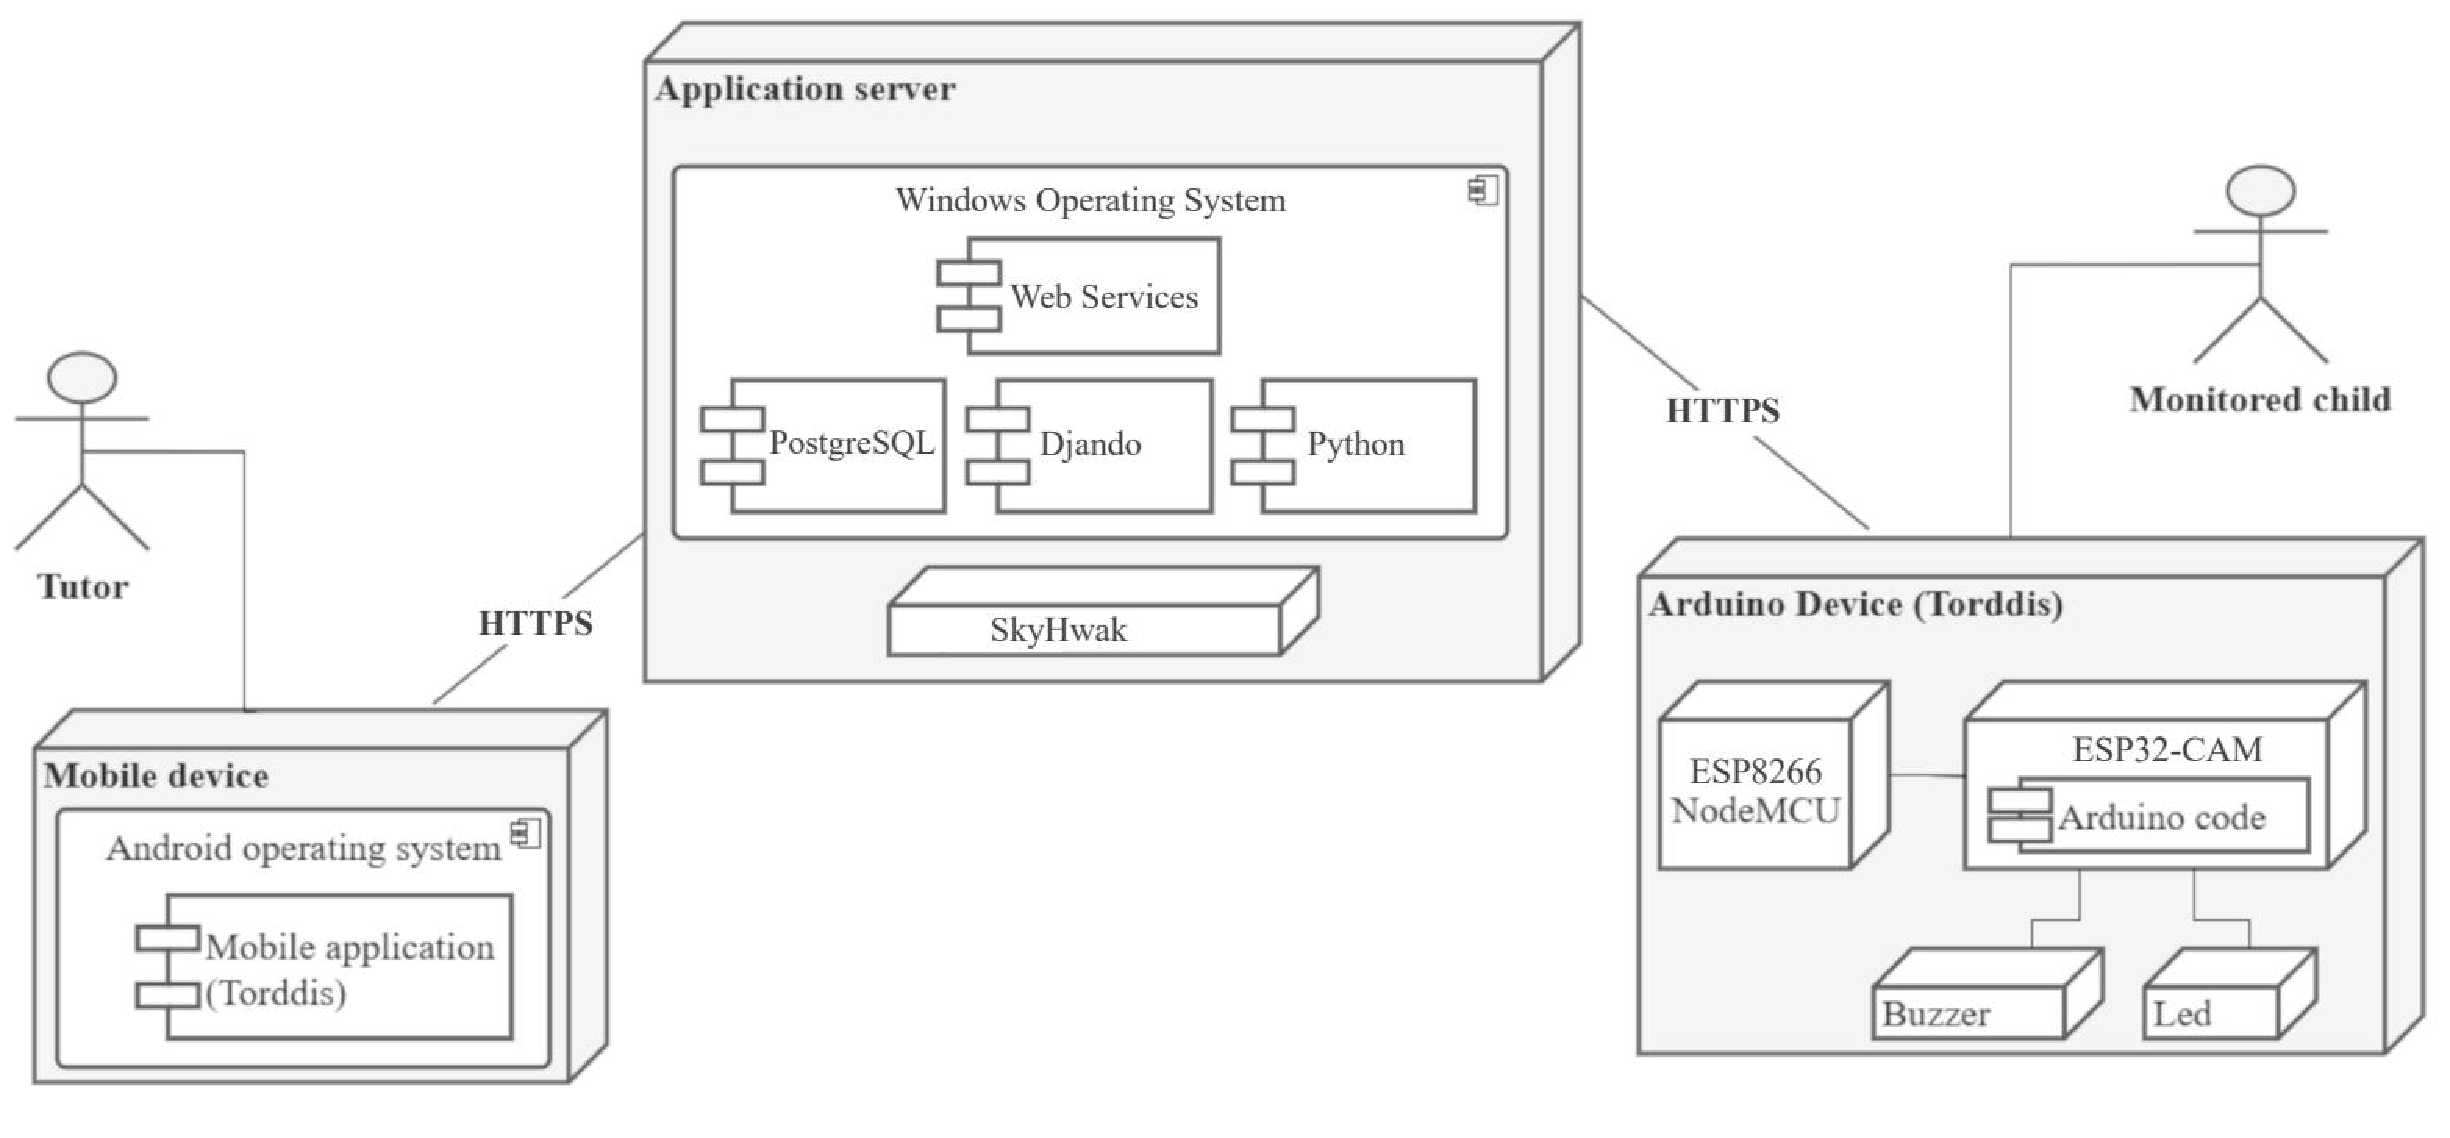
\includegraphics[frame,scale=0.5, width=0.9\linewidth]{figs/Figure_5}
                    \caption{Deployment diagram (nodes) of the Torddis system.\label{fig:TorddisArchitecture}}
                \end{figure}
                
                For the design of Torddis' architecture, given that the tutor cannot always be present beside the child during homework, the system was conceived to substitute the tutor's presence by enabling student monitoring during academic activities at home.
                
                In cases where the tutor is away from home, the architecture also considered how to inform them of the events involving the student and how they could remotely encourage the child to continue doing schoolwork. Figure~\ref{fig:TorddisDevice} illustrates the structural design of the IoT device, highlighting the components used in its construction.
                
                \begin{figure}[!htbp]
                    \centering
                    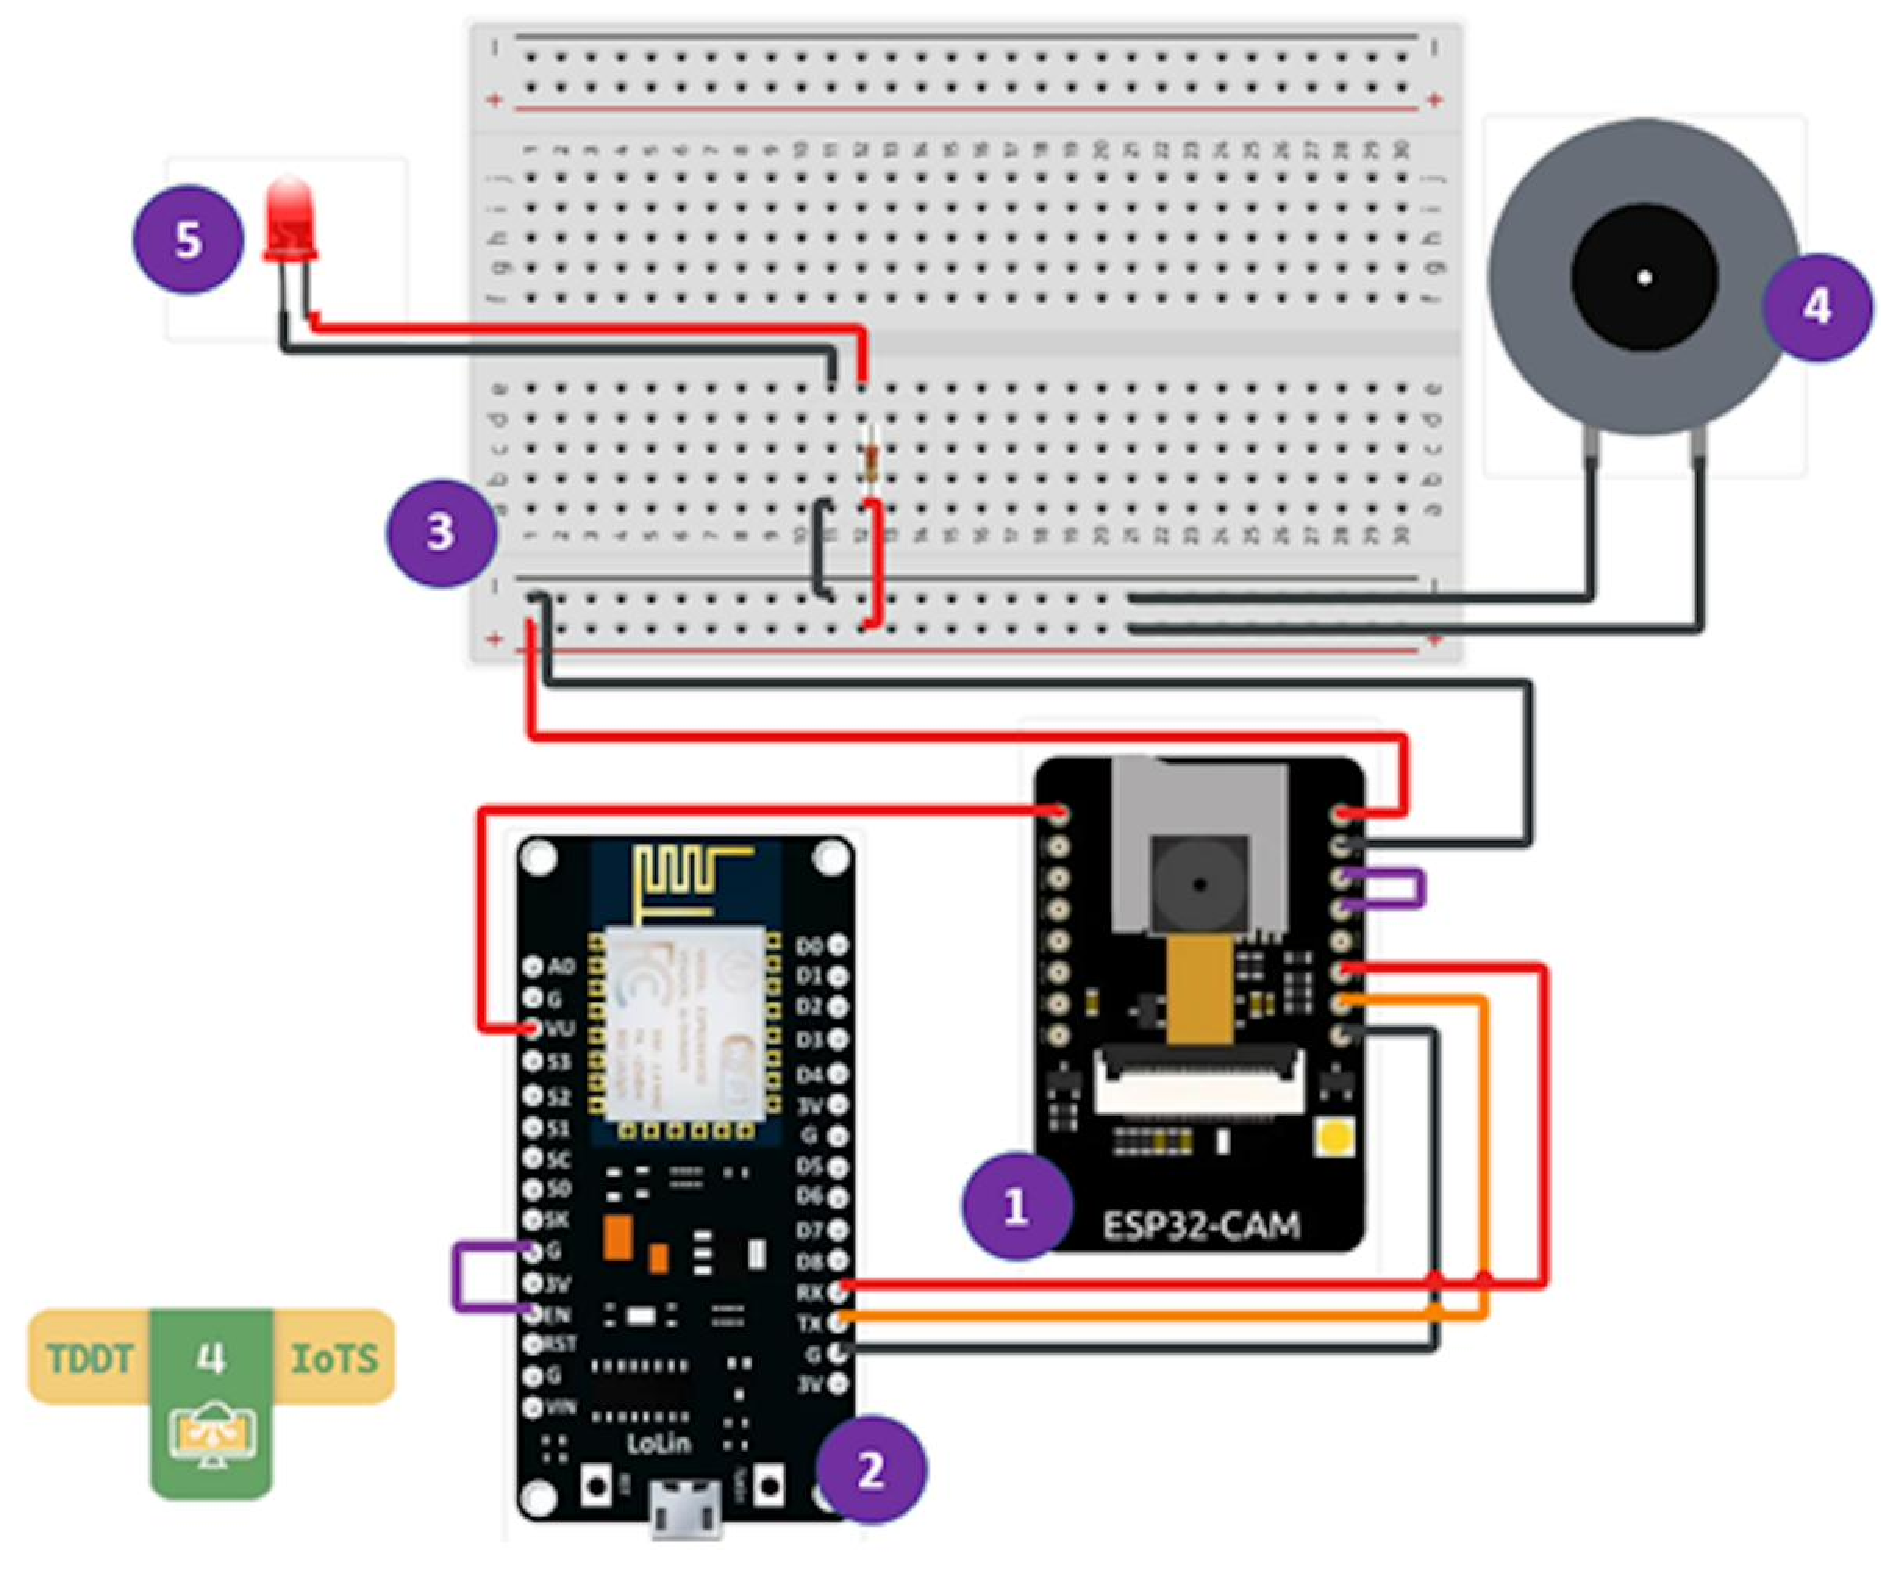
\includegraphics[frame,scale=0.5, width=0.78\linewidth]{figs/Figure_6}
                    \caption{Design of the IoT device of the Torddis system.\label{fig:TorddisDevice}}
                \end{figure}
                
                Analyzing these aspects was crucial for designing a system that supports tutors in guiding their children's learning and improving their academic performance, particularly by enhancing concentration during schoolwork at home.
                
                \subsection{Detailed Requirements Analysis}
                \label{sec:detailed-requirements}
                The requirements analysis was carried out iteratively, that is, for each of the deliverables. The two main deliverables were the IoT device and the mobile application. Furthermore, each of the components into which these deliverables were subdivided was implemented as individual tasks. These tasks spanned from two to six weeks, depending on time availability.
                
                Since the components were developed separately and sequentially, they were integrated progressively with those previously developed. Thus, upon completion of the last component, the deliverable was ready for use and testing.
                
                To detail the requirements, the process began with a literature review and was further refined based on specifications provided by future users. Each requirement listed in Table~\ref{tab:functional-requirements} and Table~\ref{tab:nonfunctional-requirements} was elaborated as a semi-structured use case that includes: (i)~unique identifier and title, (ii)~primary actor, (iii)~preconditions, (iv)~main-success scenario, (v)~alternative and exception flows, (vi)~post-conditions and (vii)~verification criteria, thereby satisfying the documentation attributes required by clause~9.4 of \citet{ISO-IEC-IEEE29148-2018}. Standardisation was further supported by \citet{Zegzhda2018Use}. A requirements-traceability matrix was maintained by the TDDT4IoTS tool linking each requirement to its use case, generated model, test case(s), and source-code artefacts, which enables both forward and backward traceability as prescribed by ISO/IEC/IEEE~29148:2018.
                
                \subsection{Model Generation and Refinement}
                Among the system modeling tools employed, structural models were used --- such as class diagrams (see Figure~\ref{fig:ClassDiagram}) --- which were generated directly by the TDDT4IoTS tool [reference anonymised] based on the use cases that specify the system to be developed.
                
                \begin{figure}[!htbp]
                    \centering
                    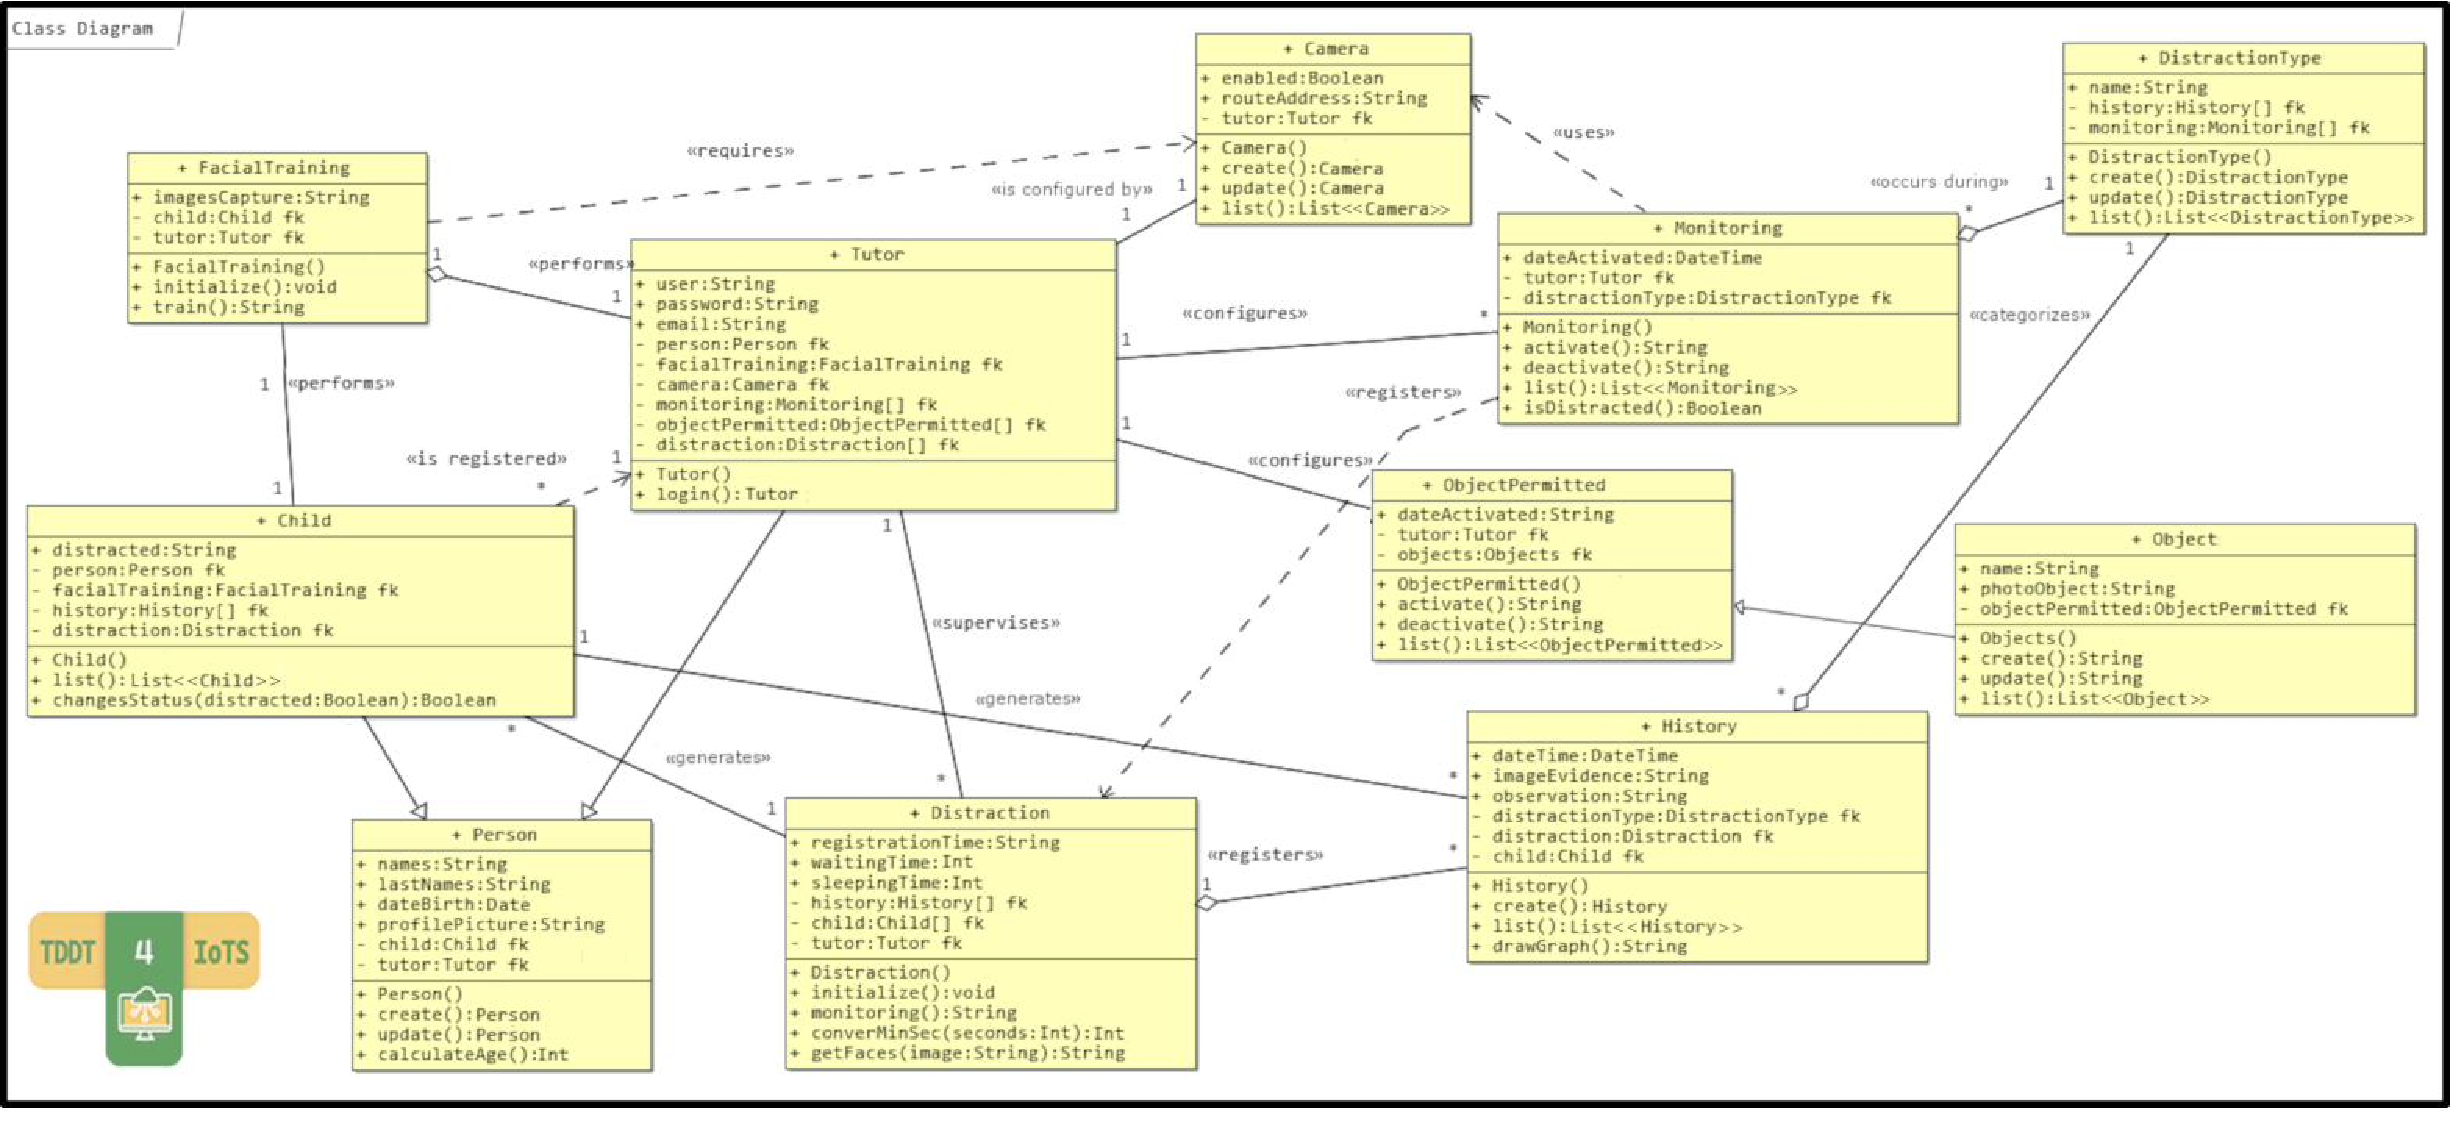
\includegraphics[frame,scale=0.5, width=\linewidth]{figs/Figure_8}
                    \caption{Class diagram of the Torddis system.\label{fig:ClassDiagram}}
                \end{figure}
                
                As TDDM4IoTS [reference anonymised] suggests that not all stages must necessarily be executed, nor in a fixed order, the model refinement stage was not applied.
                
                This stage is typically essential when requirements are unclear at the project's outset and become more defined as the development lifecycle progresses. However, in the development of Torddis, the requirements were clearly established from the beginning and remained unchanged.
                
                Furthermore, the omission of this stage is also attributable to the tool used—TDDT4IoTS [reference anonymised]—since model refinement is inherently handled within the use cases, with the tool automatically updating the models. Given that the model was generated directly from use case specifications and that Torddis did not involve a complexity level demanding extraordinary modeling efforts, the model produced by TDDT4IoTS was deemed optimal.
                
                The facial and object recognition methods implemented in the system demonstrated efficient response times and high success rates under controlled conditions. These results confirm that the system facilitates the identification of emotions and distractions, optimizing tutor intervention. This positive impact is evident in the system’s ability to reduce the need for constant supervision and improve attention and concentration during students’ schoolwork.
                
                \subsection{Test Generation}
                Test artefacts were designed and documented following the general concepts and process framework of \citet{ISO-IEC-IEEE29119-1-2022}. For each test level, a test-plan, test-design specification, test-case specification and test-execution report were produced by the TDDT4IoTS tool and are provided as Online Resource~1 (Supplementary Information). The tests required during system development are categorized as follows, and were applied to ensure that Torddis meets all previously defined requirements \citep{Sciarra2024Smash}:
                
                \begin{itemize}
                    \item \textit{Unit tests}, which are the most numerous and simplest. They allow developers to save time by detecting and correcting errors within each software code unit \citep{Mafi2024Regression}.
                    
                    \item \textit{Integration tests}, executed during the integration of components into the deliverables, ensure that interacting parts function correctly—for instance, web services with the database \citep{Spath2025Spring}.
                    
                    \item \textit{System tests}, executed when integrating all deliverables into the complete system, to verify its proper functionality \citep{Smytzek2024Tests4Py, Wang2024Ctest4J}.
                    
                    \item \textit{Acceptance tests}, conducted to evaluate the system from the end-user perspective \citep{Augusto2025Software}.
                \end{itemize}
                
                \subsection{Software Generation and Refinement}
                The software development for the Torddis system was conducted in two main stages: generation and refinement. Initially, the source code was automatically generated by the TDDT4IoTS tool [reference anonymised], based on models and tests also automatically generated from the use cases that contained the system specifications.
                
                Subsequently, this initial code was extended by developers to incorporate functionalities that could not be generated automatically by the tool.
                
                During this phase, all software components were verified by executing the pre-designed tests to ensure functionality and alignment with the established requirements.
                
                In the refinement phase, the software was improved to enhance quality and performance. Enhancements included the reduction of temporary variables through the adoption of green computing practices \citep{Firmansyah2024Integrating}, better naming conventions for attributes, methods, and classes to facilitate code readability, and the addition of comments to critical code sections. These improvements resulted in clean, maintainable, and higher-quality code, reinforcing the robustness of the Torddis system as a whole \citep{Marabesi2024Exploring}.
                
                \subsection{Hardware and Software Deployment}
                Each component of the deliverables was deployed in its designated final environment, replicating real-world conditions of the complete system. Components of the mobile application were initially tested using the Android Studio emulator. Subsequently, after generating the APK file iteratively, the mobile app was deployed on a smartphone meeting the system's minimum requirements. Figure~\ref{fig:TorddisApp} shows screenshots of the deployed mobile application and the corresponding IoT device.
                
                \begin{figure}[!htbp]
                    \centering
                    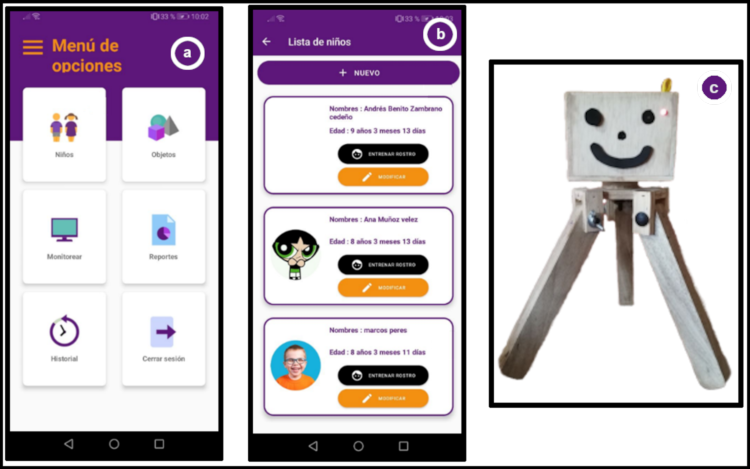
\includegraphics[width=\linewidth]{figs/Figure_9}
                    \caption{Screenshots of the mobile application and the Torddis system device.\label{fig:TorddisApp}}
                \end{figure}
                
                The components of the final IoT device (Torddis system) were iteratively and incrementally deployed in simulated or testing environments during development phases. Later, for integration and system tests, the system was deployed in an ideal real-world environment where any student could perform schoolwork.
                
                Functional hardware and software tests validated system performance under optimal conditions, ensuring proper integration among technological components. Nevertheless, additional testing was deemed necessary in adverse scenarios such as environments with low connectivity or high ambient noise. These situations will allow evaluation of the system’s robustness and expand its applicability to more challenging real-life contexts \citep{Falzetti2024Promoting}.
                
                \subsection{System Artefacts and Selected Technologies}
                \label{sec:torddis-artefacts}
                Table~\ref{tab:Roles} listed the team roles; this subsection summarises the concrete artefacts produced during the preliminary and technological-layer stages: the coarse-grained use case model, the selected hardware components, the selected software technologies and the distraction parameters that the AI modules must monitor. These artefacts drive the study design reported in Section~\ref{section:fifth} and the results reported in Section~\ref{section:sixth}.
                
The coarse-grained analysis of the functional requirements is presented in the general use case diagram shown in Figure~\ref{fig:UseCaseDiagram}. These functionalities and their corresponding actors were identified as a result of the initial interviews with the end user (a guardian).
                
                \begin{figure}[!htbp]
                    \centering
                    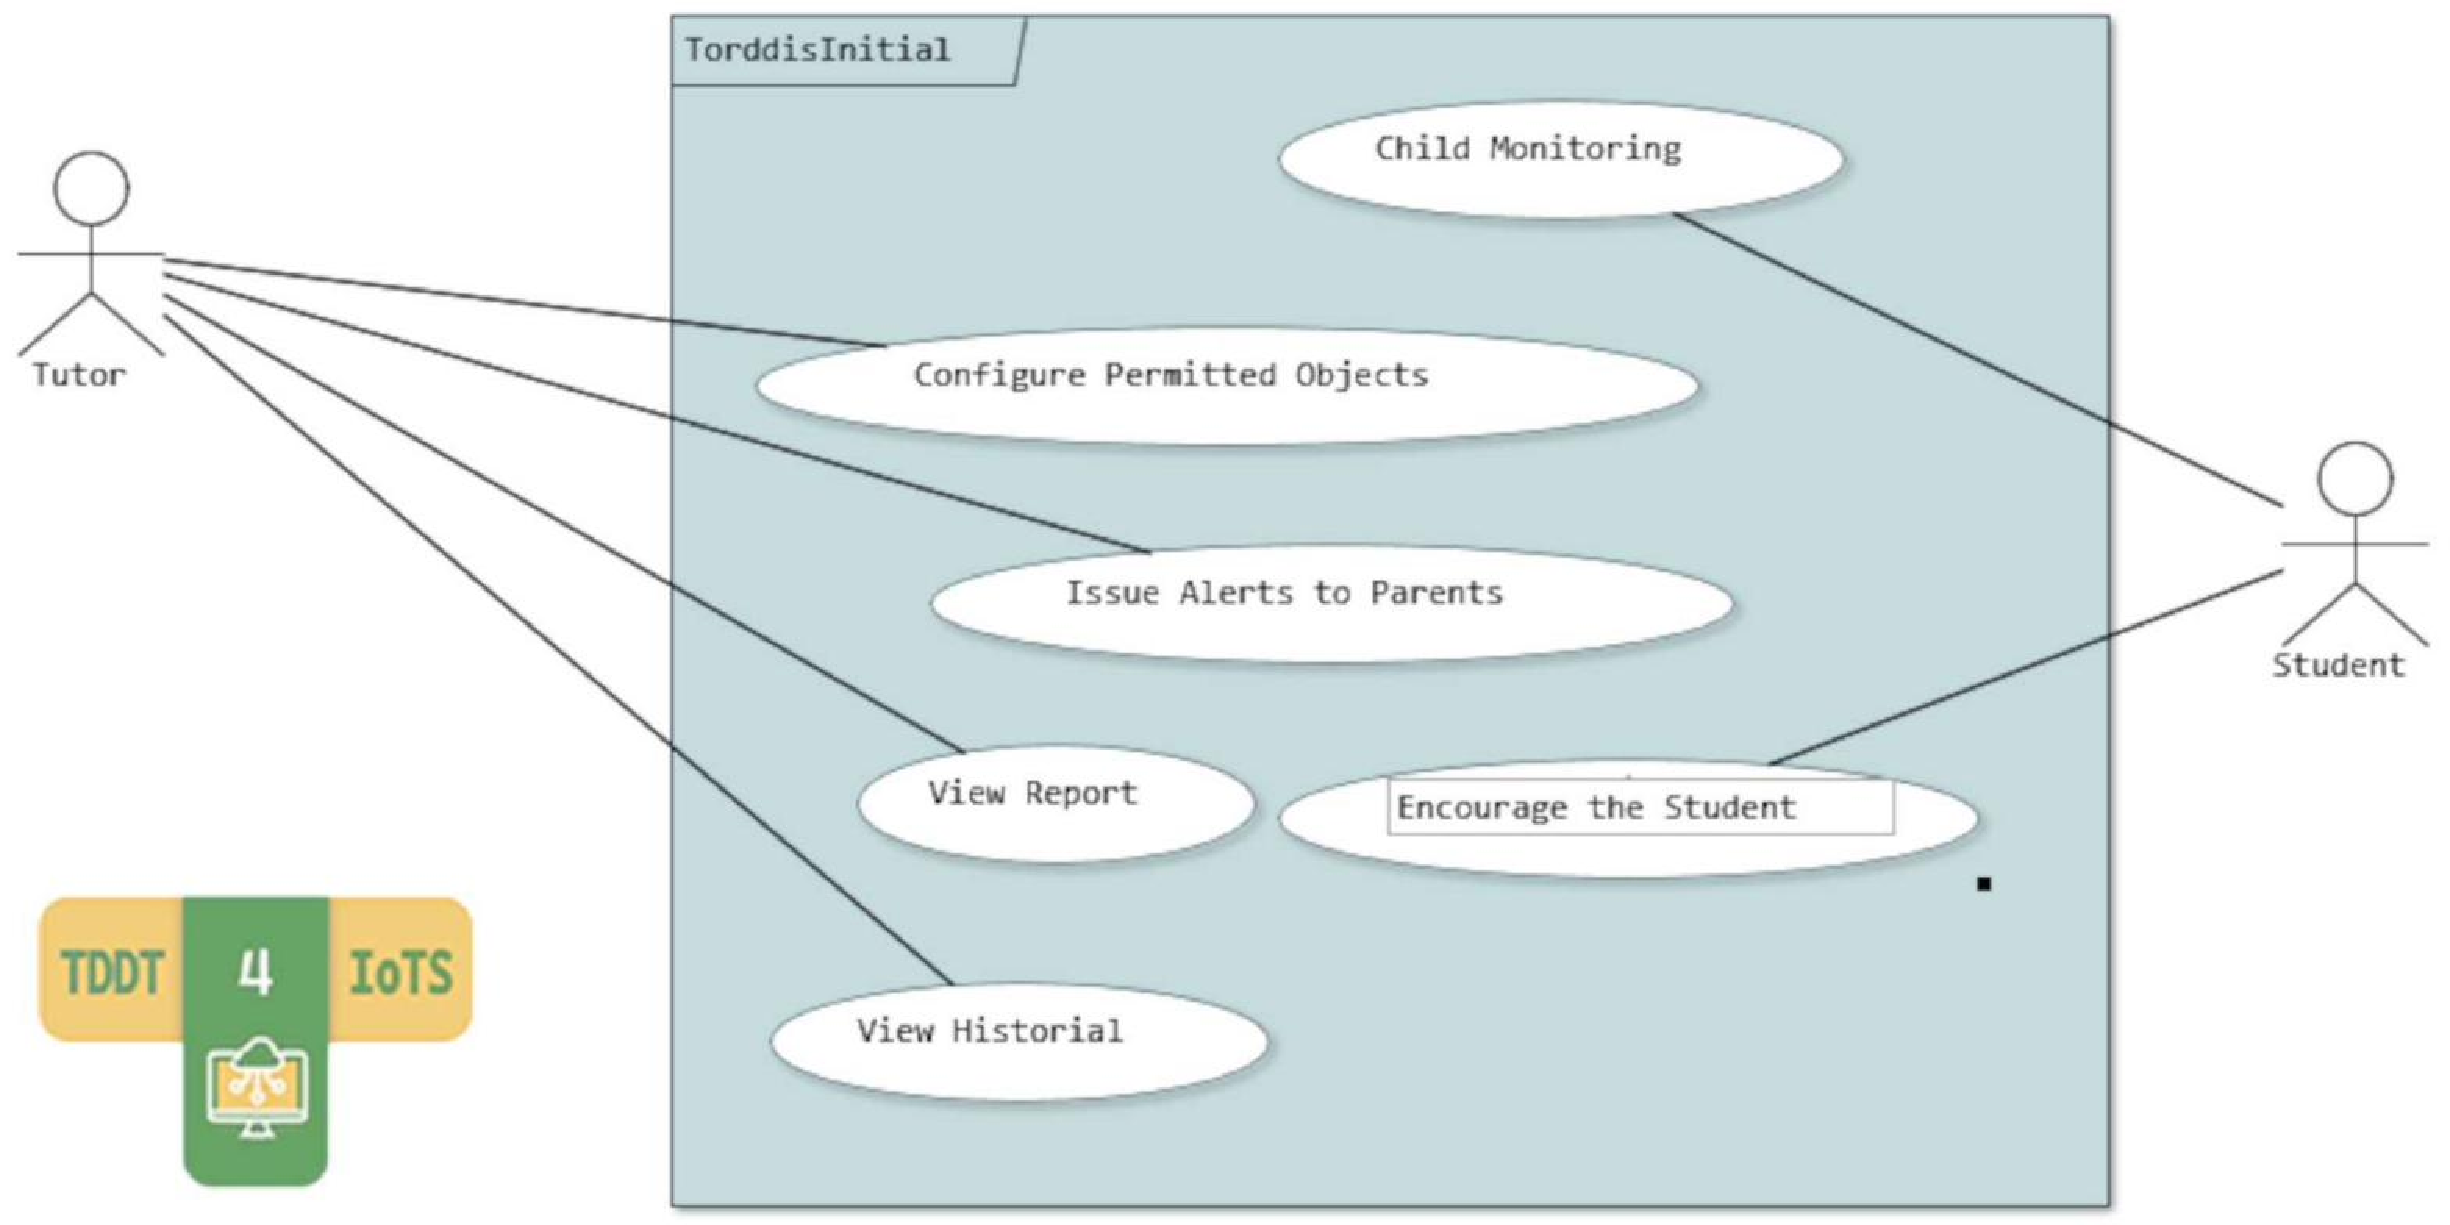
\includegraphics[frame,scale=0.5, width=\linewidth]{figs/Figure_2.pdf}
                    \caption{High-level user requirements modeling.\label{fig:UseCaseDiagram}}
                \end{figure} 
                
                The \textit{guardian} user is responsible for configuring the \textit{allowed objects}, \textit{monitoring} their \textit{students}, receiving alerts issued by the system regarding detected events, and persuading the monitored student to remain focused. Additionally, the guardian can access system-generated reports and review the history of recorded events.
                
                \subsubsection{Hardware Resources}
                The hardware used for building the Torddis system device was selected based on criteria of integration, low power consumption, and compatibility with real-time monitoring environments. Table~\ref{table:hardware-components} presents the main components employed, along with their corresponding functionalities, evaluated alternatives, and technical remarks. The ESP32-CAM and NodeMCU ESP8266 modules stand out due to their wireless connectivity and embedded processing capabilities, making them suitable for video transmission and information exchange with the web service. Furthermore, peripheral components such as passive buzzers and 5 mm LEDs were incorporated to emit auditory and visual alerts, thereby fulfilling the system’s functional requirements for home-based educational supervision.
                
                \begin{table}[!htbp]
                    \caption{Selected hardware components and technical observations}
                    \label{table:hardware-components}
                    \centering
                                            \begin{tabular}{
                                >{\raggedright\arraybackslash}p{0.25\textwidth}
                                >{\raggedright\arraybackslash}p{0.12\textwidth}
                                >{\raggedright\arraybackslash}p{0.15\textwidth}
                                >{\raggedright\arraybackslash}p{0.48\textwidth}
                            }
                            \toprule
                            \multicolumn{1}{c}{\textbf{Functionality}} &
                            \multicolumn{1}{c}{\textbf{Selected}} &
                            \multicolumn{1}{c}{\textbf{Alternatives}} &
                            \multicolumn{1}{c}{\textbf{Technical Observation}} \\
                            \midrule
                            Web service connectivity and video streaming & ESP32-CAM & OV7670 VGA camera & This module includes Wi-Fi + Bluetooth connectivity and an integrated video camera \citep{CasasSanchez2022}. \\
                            Data transmission & NodeMCU ESP8266 v3 & Arduino UNO, GSM module & The NodeMCU is a compact board that provides Wi-Fi connectivity for data transmission to the web service \citep{Barai2019}. \\
                            Alarm sound emitter & Passive buzzer & Active buzzer & Commonly used to generate audible alerts in electronic boards \citep{Adebisi2023development}. \\
                            Visual alert emitter & 5mm LED (any color) & RGB LED & Bright clear LED diode used to provide visual alerts \citep{Upender2020}. \\
                            \bottomrule
                        \end{tabular}
                    
                \end{table}
                
                \subsubsection{Software Technologies}
                The system's development enabled the effective integration of diverse technologies, including programming languages and AI algorithms, which facilitated the achievement of the proposed objectives and demonstrated its technical feasibility. Table \ref{table:software-technologies} presents the software technologies used in the development of the Torddis system.
                
                \begin{table}[!htbp]
                    \caption{Software technologies used in the development of the Torddis system}
                    \label{table:software-technologies}
                    \centering
                                            \begin{tabular}{
                                >{\raggedright\arraybackslash}p{0.25\textwidth}
                                >{\raggedright\arraybackslash}p{0.12\textwidth}
                                >{\raggedright\arraybackslash}p{0.15\textwidth}
                                >{\raggedright\arraybackslash}p{0.48\textwidth}
                            }
                            \toprule
                            \multicolumn{1}{c}{\textbf{Functionality}} &
                            \multicolumn{1}{c}{\textbf{Selected}} &
                            \multicolumn{1}{c}{\textbf{Alternatives}} &
                            \multicolumn{1}{c}{\textbf{Technical Observation}} \\
                            \midrule
                            
                            Android mobile application & Java & Kotlin & Language used in Android Studio, with a large developer community in the mobile application domain \citep{Sharma2021Real-Time}. \\
                            
                            AI applications & Python & Java, R & Programming language with popular open-source libraries for AI application development \citep{Cai2005OnThePerformance}. \\
                            
                            Web applications and services & Django & Flask & Popular framework with rapid development capabilities that helps prevent security flaws in web applications and services \citep{Puneet2022ADjango}. \\
                            
                            Databases & PostgreSQL & MySQL, MariaDB, Firebird & Robust database with enhanced compatibility with the Django web framework \citep{Puneet2022ADjango}. \\
                            
                            \bottomrule
                        \end{tabular}
                    
                \end{table}
                
                \subsubsection{Distraction Parameters}
                The distraction parameters identified in the literature as factors affecting children's concentration during academic activities were refined based on user feedback and expert input from an education professional. Table \ref{tab:DistractionParameters} summarizes the distraction parameters that were defined by consensus.
                
                \begin{table}[!htbp]
                    \centering
                    \caption{Distraction parameters identified in the study area \label{tab:DistractionParameters}}
                    \begin{tabularx}{\linewidth}{@{}
                            >{\raggedright\arraybackslash}X
                            >{\raggedright\arraybackslash}X @{}}
                        \toprule
                        \multicolumn{1}{c}{\textbf{Internal Distraction}} &
                        \multicolumn{1}{c}{\textbf{External Distraction}} \\
                        \midrule
                        Emotional expressions such as anger, disgust, fear, happiness, sadness, surprise, and neutral state \citep{Asish2022Detecting,Vettivel2018System,Pabba2022AnIntelligent}. &
                        Intervention of an unfamiliar person or abandonment of the study area \citep{Vettivel2018System}. \\
                        Drowsiness state to determine whether the child is awake or asleep \citep{Pabba2022AnIntelligent}. &
                        Presence of objects in the study area that divert attention from the ongoing academic tasks \citep{Asish2022Detecting,Pabba2022AnIntelligent}. \\
                        \bottomrule
                    \end{tabularx}
                \end{table}
                
                \subsection{Standards Compliance and Ethical Considerations}
                \label{sec:standards-compliance}
                Table~\ref{tab:standards-compliance} summarises the international standards followed during the Torddis life cycle and the artefacts through which the corresponding conformance is materialised.
                
                \begin{table}[!htbp]
                    \centering
                    \caption{International standards followed during the Torddis life cycle and corresponding artefacts.\label{tab:standards-compliance}}
                    \begin{tabular*}{\linewidth}{@{\extracolsep{\fill}}
                            >{\raggedright\arraybackslash}p{4.4cm}
                            >{\raggedright\arraybackslash}p{4.2cm}
                            >{\raggedright\arraybackslash}p{4cm}
                            @{}}
                        \toprule
                        \multicolumn{1}{c}{\textbf{Standard}} & \multicolumn{1}{c}{\textbf{Scope of application}} & \multicolumn{1}{c}{\textbf{Corresponding artefact(s)}} \\
                        \midrule
                        ISO/IEC/IEEE 12207:2017 \citep{ISO-IEC-IEEE12207-2017} & Software life-cycle processes & TDDM4IoTS phases, source code \\
                        ISO/IEC/IEEE 15288:2023 \citep{ISO-IEC-IEEE15288-2023} & System life-cycle processes & Preliminary and feasibility analyses \\
                        ISO/IEC/IEEE 29148:2018 \citep{ISO-IEC-IEEE29148-2018} & Requirements engineering & Tables~\ref{tab:functional-requirements}, \ref{tab:nonfunctional-requirements}; use cases; traceability matrix \\
                        ISO/IEC 25010:2023 \citep{ISO-IEC25010-2023} & Product quality model & Non-functional requirements classification (Table~\ref{tab:nonfunctional-requirements}) \\
                        ISO/IEC/IEEE 42010:2022 \citep{ISO-IEC-IEEE42010-2022} & Architecture description & Deployment view (Figure~\ref{fig:TorddisArchitecture}); logical view (Figure~\ref{fig:ClassDiagram}) \\
                        ISO/IEC/IEEE 29119-1:2022 \citep{ISO-IEC-IEEE29119-1-2022} & Software testing --- General concepts & Test plan and cases in Online Resource~1 \\
                        ISO/IEC 27001:2022 \citep{ISO-IEC27001-2022} & Information security management & NFR-04 (end-to-end encryption of personal data) \\
                        \bottomrule
                    \end{tabular*}
                \end{table}
                
                Because the study involved children as data subjects, the protocol was reviewed and approved by the Research Committee of the Faculty of Engineering Sciences (the participating public university). Written informed consent was obtained from every guardian on behalf of the child; children over ten years old provided verbal assent. All personal data were pseudonymised at capture, stored encrypted at rest and in transit, and were accessed only by the two authors responsible for the statistical analysis. The study adheres to the principles of the Declaration of Helsinki and to the data-protection provisions applicable in the participants' jurisdiction, aligned with \citet{ISO-IEC27001-2022}.
                
                \section{Methodological Design of the Study and Experimental Validation}
                \label{section:fifth}
                This study is based on a methodological approach that seeks to establish a bridge between technological design and pedagogical processes, with the aim of rigorously evaluating the impact of Torddis in real-world usage contexts. This section outlines the validation strategy employed, understood not only as a technical phase but as a key instance for articulating theory, user experience, and empirical evidence. The adopted methodological structure responds to both scientific validity requirements and the need to generate applicable knowledge in dynamic and diverse educational environments.
                
                \subsection{Participants and Study Context}
                The study involved 12 children and their respective guardians, selected through convenience sampling. The children, aged between 7 and 12 years, were enrolled in primary and lower secondary education. The guardians, aged between 25 and 65, had primary and secondary education levels. Participants resided in both urban and rural areas with access to basic services (electricity, drinking water, internet, and mobile telephony).
                
                The selection criteria ensured that households had access to home internet (Wi-Fi or mobile data) and mobile data on the guardian’s smartphone, which were necessary conditions for system deployment. This approach ensures that the participants reflect the profile of potential Torddis users: families with guardians engaged in activities inside and outside the home, responsible for school-aged children requiring supervision.
                
                The representativeness of the sample is considered acceptable given that real users of the system were involved and the defined inclusion criteria were met. Convenience sampling is appropriate for preliminary investigations such as this, allowing the collection of significant data despite limited availability or willingness of families to participate \citep{DiPietro2025Meta}.
                
                \subsection{Experimental Process and Instrument Validation}
                The experimental process was conducted in two phases, which are described in the following subsections.
                
                \subsubsection{Controlled Environment}
                This phase was designed to evaluate the system’s usability and performance. During the evaluation, guardians used the Torddis prototype with their children for 30 minutes in a previously prepared environment where all system functionalities were verified. To collect user experience data, SUS-type questionnaires and open-ended questions were administered.
                
                \subsubsection{Real Environment}
                This phase aimed to evaluate system effectiveness. It lasted one week, considering that only a single prototype was available. A Likert-scale questionnaire was used to assess guardians' perceptions of the system’s utility and effectiveness (see Appendix \ref{Appendix:LikertEffectivity}), including questions on device attractiveness, notification accuracy, and its impact on children's self-regulation and concentration \citep{Ackermans2025Young}.
                
                Instrument validity was ensured through expert review, confirming the clarity and relevance of the questions for the study’s purpose. In addition, system-generated data (e.g., detection of distracting objects and alerts) were manually verified to guarantee accuracy \citep{Wang2025Development}. The data were also analyzed to determine whether the variables followed a normal distribution, thereby guiding the choice of appropriate statistical methods (ANOVA, Kruskal–Wallis) and correlation coefficients (Pearson and Spearman).
                
                \subsection{Randomization and Bias Control}
                No randomization process was implemented due to the nature of the convenience sample. However, the following measures were adopted to minimize bias \citep{Huang2025How}:
                
                \begin{itemize}
                    \item Detailed explanation of each questionnaire item before participant completion.
                    
                    \item Assurance of anonymity and confidentiality of responses.
                    
                    \item Questionnaire administration without the presence of researchers to avoid influencing responses.
                \end{itemize}
                
                Nonetheless, potential bias related to the researchers’ proximity to participants is acknowledged, which may have influenced the responses \citep{DiPietro2025Meta}.
                
                \subsection{Instruments and Statistical Analysis}
                To evaluate the effectiveness of the Torddis system, validated instruments and statistical tests were used to analyze guardians’ perceptions as well as improvements in students’ self-regulation and concentration. Collected data included questionnaire responses and system-generated metrics, allowing an integrated analysis combining subjective and objective perspectives.
                
                \subsubsection{Questionnaires and Scales}
                Three main questionnaires were used to assess various aspects of the Torddis system, in addition to the demographic survey:
                
                \begin{itemize}
                    \item A standard \textbf{System Usability Scale (SUS)} questionnaire consisting of 10 items (see Appendix \ref{Appendix:SUSLikertQuestionary}) to assess overall system usability from the guardians’ perspective. A specific preprocessing procedure was followed: negatively worded items were reverse scored, and final results were scaled from 0 to 100, in accordance with SUS guidelines \citep{Brown1989}, ensuring score comparability and alignment with international usability benchmarks.
                    
                    \item An open-ended questionnaire (see Appendix \ref{Appendix:SUSOpenQuestionarie}), used to identify areas for improvement before finalizing the system, allowing feedback on usability and effectiveness.
                    
                    \item A Likert-type questionnaire with seven statements (see Appendix \ref{Appendix:LikertEffectivity}), designed to measure \textit{guardians’ perceptions of system effectiveness} in the home setting. Statements evaluated aspects such as device attractiveness (\textit{Statement 1}), discretion during use (\textit{Statement 3}), and perceived improvements in self-regulation and concentration after use (\textit{Statement 5}). This instrument was validated by a panel of experts for clarity and relevance.
                \end{itemize}
                
                The integration of these instruments’ data with system-generated metrics enabled a more robust analysis. Collected metrics included:
                
                \begin{itemize}
                    \item Frequency and duration of homework supervision by guardians.
                    
                    \item Number of system alerts issued to redirect student attention.
                    
                    \item Effective device usage time during homework activities.
                \end{itemize}
                
                Data collected by the Torddis system, such as alert frequency and active supervision time, were incorporated into the statistical analysis to support qualitative findings. Additionally, usage pattern analysis reinforced the validity of guardians’ perceptions regarding system effectiveness and usefulness.
                
                This comprehensive statistical approach ensures that the results accurately reflect the impact of the Torddis system on children's supervision dynamics while completing homework, providing a solid foundation for future improvements and deployments.
                
                \subsubsection{Statistical Analysis}
                Descriptive and analytical statistical analyses were performed to validate the collected data, including:
                
                \begin{itemize}
                    \item \textbf{Descriptive statistics:} Measures of central tendency (mean) and dispersion (standard deviation) were calculated for each statement in the Likert scale, revealing general patterns in guardians' perceptions \citep{Yaska2024Assessment}.
                    
                    \item \textbf{Normality tests:} Shapiro–Wilk \citep{Souza2023Sample} and Kolmogorov–Smirnov \citep{Lilliefors1969Kolmogorov} tests were applied to assess the distribution of numerical variables. Results determined whether parametric or non-parametric tests were used.
                    
                    \item \textbf{Correlations:} Pearson \citep{Yu2024Inferential} and Spearman \citep{Yu2024Robust} correlation coefficients were computed to explore relationships between questionnaire statements on system effectiveness \citep{Jebb2021Review}. For example, \textit{Statement 5} showed significant correlations with statements on device attractiveness (\textit{Statement 1}) and discretion (\textit{Statement 3}).
                    
                    \item \textbf{Qualitative analysis:} Open-ended responses and SUS Likert responses were analyzed alongside system metrics to identify cases where guardians’ qualitative perceptions complemented or contradicted quantitative data.
                    
                    \item \textbf{Analysis of variance (ANOVA):} ANOVA was applied \citep{Dubey2025Two,Rojas2025Validating} to assess differences in perception based on guardians’ demographic characteristics, such as educational level or place of residence (urban/rural), identifying contextual influences on system perception.
                \end{itemize}
                
                \subsection{Limitations and Generalization}
                The study has certain limitations:
                
                \begin{enumerate}
                    \item The sample was limited to a small group selected via convenience sampling, which may not represent other sociodemographic or technological contexts.
                    
                    \item The real-world phase lasted only one week, limiting the assessment of the system’s long-term impact on self-regulation skills.
                    
                    \item Only one prototype was available, restricting simultaneous use by multiple participants.
                \end{enumerate}
                
                These limitations are common in pilot or early-stage studies exploring educational technology impact.
                
                Previous studies have highlighted that the generalizability of results from technological interventions strongly depends on population characteristics and implementation context. For example, a recent meta-analysis on the effects of technology on disadvantaged students emphasizes how resource access and contextual conditions can significantly influence outcomes. It recommends designing future studies with broader and more diverse populations to enhance representativeness \citep{DiPietro2025Meta}.
                
                \subsection{Validation of the TDDM4IoTS Methodology}
                The TDDM4IoTS methodology [reference anonymised] was selected for its focus on IoT projects, enabling iterative hardware–software integration. During Torddis development, this methodology supported:
                
                \begin{itemize}
                    \item Definition of functional and non-functional requirements based on guardian needs.
                    
                    \item Automated test generation, reducing development time and errors.
                    
                    \item Early component validation, ensuring system robustness.
                \end{itemize}
                
                Compared to traditional methodologies, TDDM4IoTS stands out for its adaptability to projects with multiple interdependent deliverables, such as those combining diverse IoT components and mobile applications. Furthermore, it ensures compliance with system lifecycle standards [reference anonymised].
                
                Structured methodologies (such as TDDM4IoTS) are particularly effective in the development of technology-based educational systems, as they efficiently integrate technological and pedagogical components \citep{Borte2024Learning,Kirkwood2014Technology}. According to recent studies on adaptive learning systems, applying clear methodological frameworks not only ensures robust development but also aligns system features with users’ specific needs. This methodological approach is key to addressing interoperability and personalization challenges in educational contexts \citep{Wang2025Development}.
                
                \subsection{Pedagogical Justification}
                The system design and applied methodology align with key pedagogical goals, such as fostering self-regulation and autonomous learning skills in students. Through immediate feedback and personalization, Torddis helps students manage attention and time, while guardians can supervise and support the learning process \citep{Chen2025Unpacking}.
                
                Moreover, the iterative development stages guided by TDDM4IoTS allowed for the incorporation of pedagogical improvements at each phase, ensuring the system addresses both technological and educational needs \citep{Huang2025How}.
                
                \section{Results}
                \label{section:sixth}
                This section presents the empirical results of the Torddis pilot evaluation. Two dimensions are reported: (i)~the usability of the mobile application and IoT device, as perceived by the guardians who supervised its use at home, and (ii)~the technical performance of the AI recognition modules under real-world operating conditions. The complementary statistical analyses of the guardians' effectiveness questionnaire are presented in Subsection~\ref{sec:stats-analysis}.
                \subsection{Deliverable Evaluation}
                Each deliverable (mobile application and device) was evaluated by the user in an ideal setting. Figure~\ref{fig:ConfigEvaluation} shows the configuration of one of the environments used to evaluate the Torddis system. The child is seated at a desk performing school tasks while being monitored by the Torddis system.
                
                \begin{figure}[!htbp]
                    \centering
                    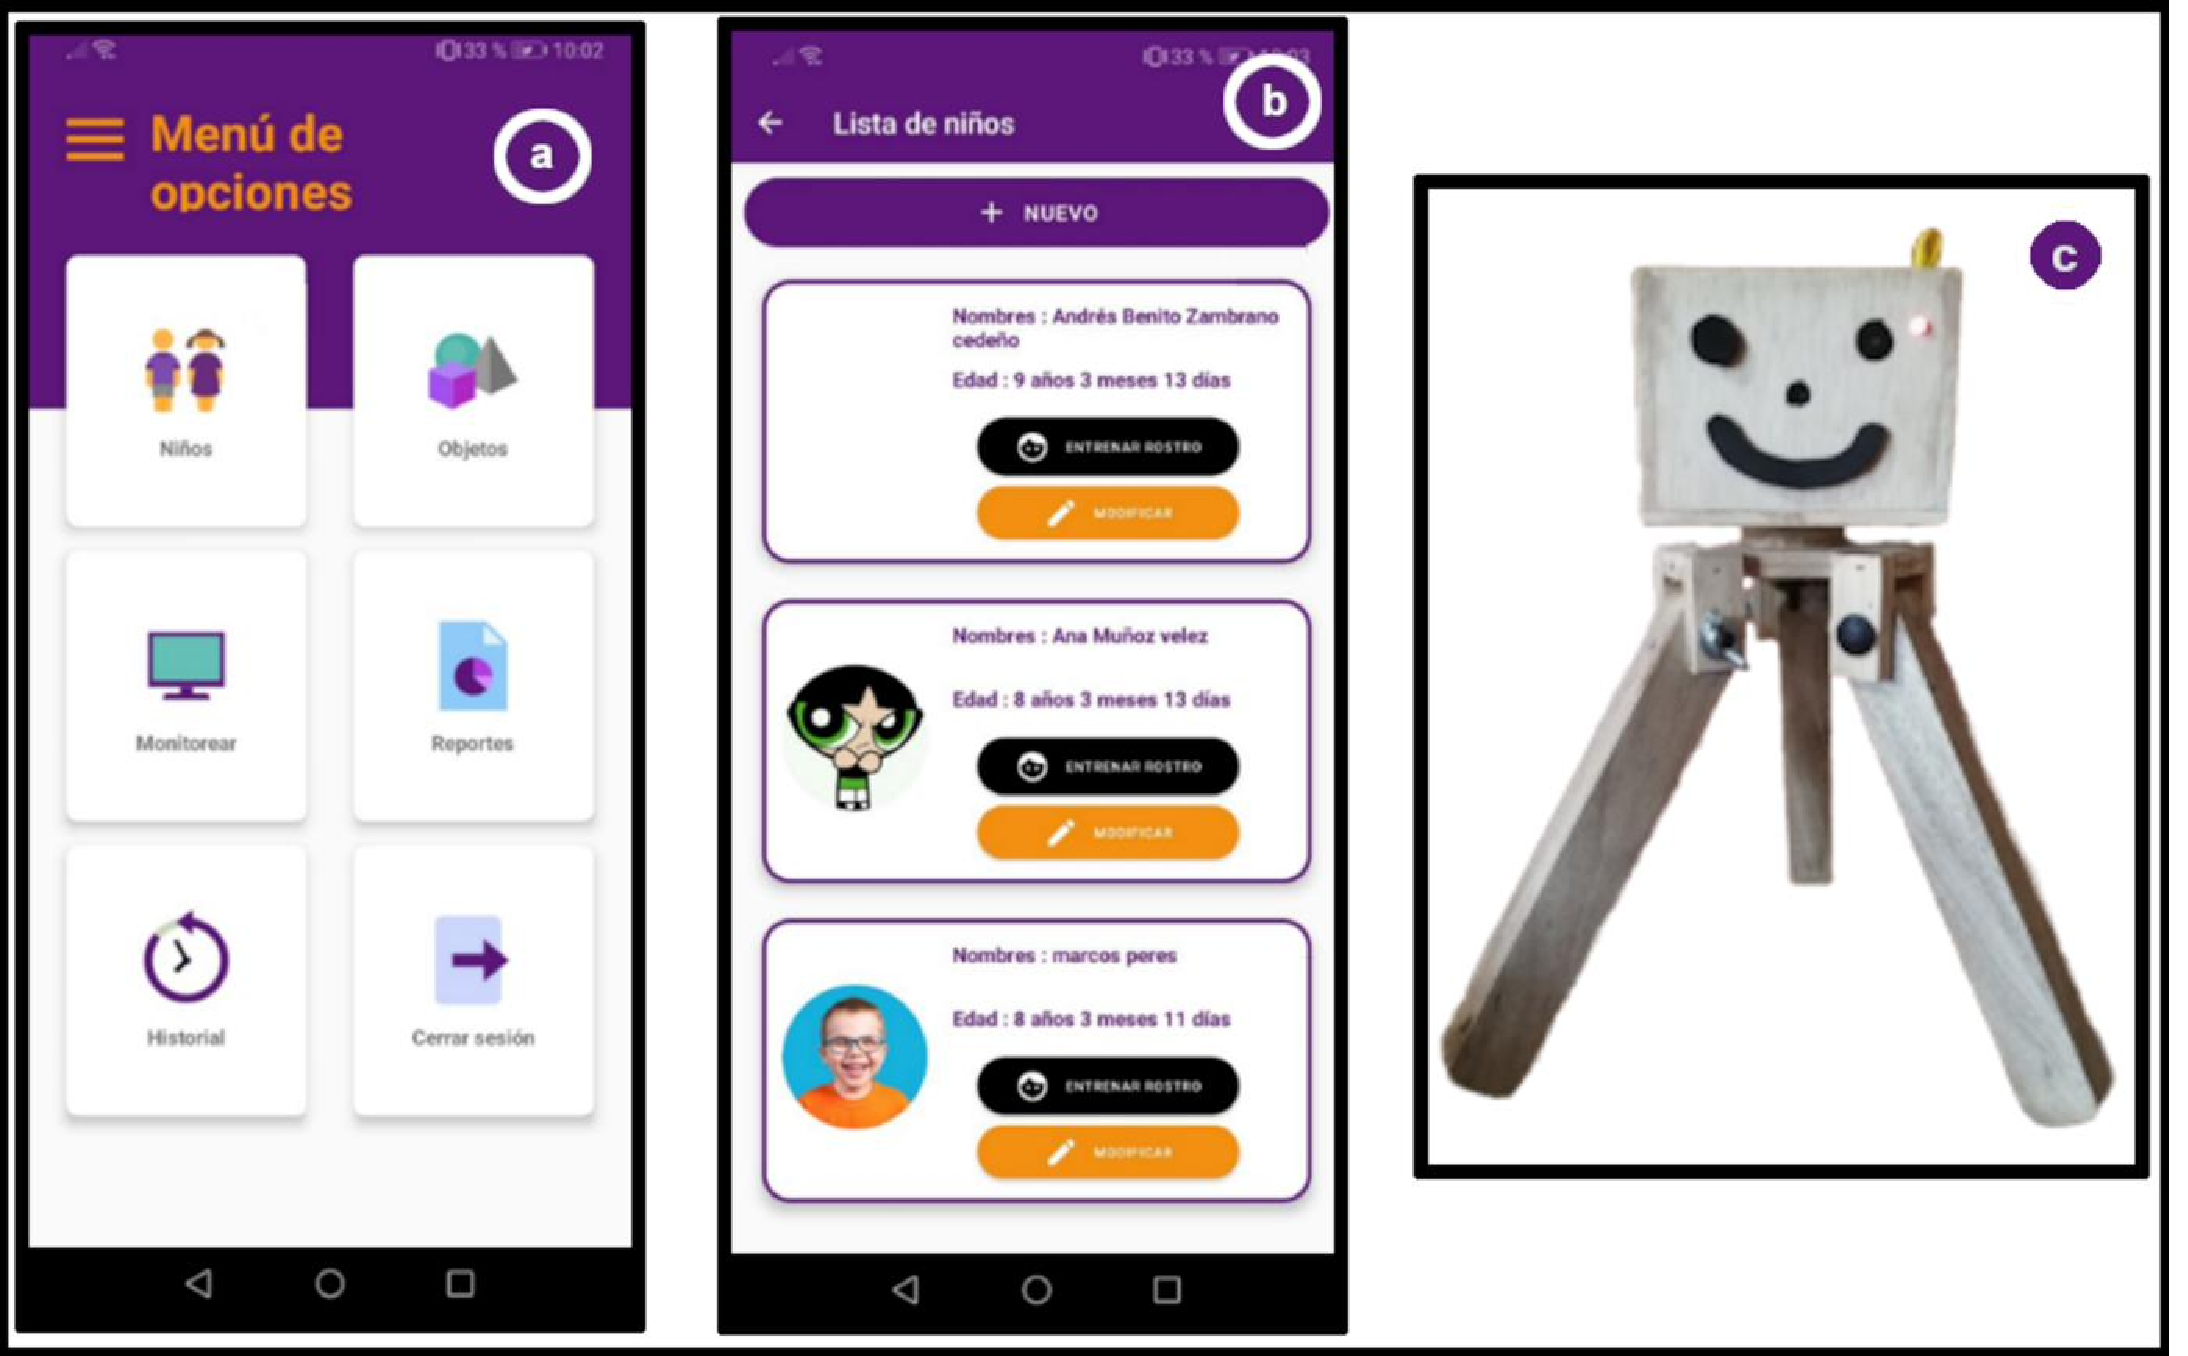
\includegraphics[width=\linewidth]{figs/Figure_10}
                    \caption{Setup of the environment for evaluating the Torddis system.\label{fig:ConfigEvaluation}} 
                \end{figure}
                
                The system is capable of monitoring the student’s concentration and identifying distractions. The device is placed at a distance of 50 to 70 cm from the child to ensure optimal camera operation, which provides the necessary input for facial recognition and object detection technologies. It is worth noting that, from the child’s perspective, the device is intended to be perceived as a decorative item on the desk.
                
                An evaluator (one of the authors of this article), along with one or both parents, is present (seated in front of the TV). They are positioned approximately three meters from the child. The evaluator supervises the system’s operation via a laptop, while the parent(s) use the mobile application integrated with the IoT device to monitor the child’s concentration in real time.
                
                This setup allowed for a comprehensive evaluation of the Torddis system, ensuring that all involved parties (children, parents, and evaluators) could interact with the technology and provide valuable feedback on its effectiveness in monitoring and enhancing concentration during academic activities.
                
                To evaluate the system's functionalities as a whole, five acceptance test cases were designed and executed, covering tutor account creation, login, facial training, device registration, and configuration of monitored objects. Their detailed specifications --- following the guidelines of \cite{Sciarra2024Smash} --- are provided as Online Resource~1 (Supplementary Information, Section~S1).
                
                \subsubsection{Usability Evaluation of the Developed System Prototype}
                The usability evaluation of the Torddis system was conducted to collect information about the overall user experience, focusing specifically on ease of use, interface design, and the effectiveness of the features provided. This comprehensive evaluation aimed to identify strengths and areas for improvement, ensuring that the system effectively meets user needs. The following subsections detail the demographic data of the participants, their experiences, the specific tasks performed during the evaluation, and the results obtained through the use of Likert-scale questionnaires (see Appendix~\ref{Appendix:SUSLikertQuestionary}) and open-ended questions (see Appendix~\ref{Appendix:SUSOpenQuestionarie}) from the System Usability Scale (SUS) \citep{Brooke1996SUS}.
                
                \paragraph{Demographic Data.}
                At the beginning of the usability evaluation of the Torddis system, a demographic questionnaire was provided (see Appendix~\ref{Appendix:DemographicSurvey}) to gather information about the tutors who participated in the evaluation. The questionnaire yielded the following results:
                
                \begin{itemize} 
                    \item A total of 12 families were evaluated, represented by 8 mothers and 4 fathers, all from the geographic area of a Latin American educational setting.
                    \item The average age of the participants was 39 years, ranging from 25 to 65 years.
                    \item 58\% of the tutors had completed only primary education, while 42\% had reached secondary education.
                \end{itemize}
                
                \paragraph{About Monitoring.}
                One of the preliminary questions in the usability evaluation focused on how easily the tutors could monitor their children while performing school tasks. Most tutors responded that monitoring for signs of distraction during homework was a complex task, as shown in Figure~\ref{fig:monitoring-process}, which presents the responses to that question. Another question asked about how frequently they needed to monitor their children during such activities. Most tutors indicated that they had to do so constantly (as shown in Figure~\ref{fig:monitoring-frequency}). Finally, tutors reported that among the strategies they use to help their children stay focused during school activities are scolding, motivational advice, and rewards such as candies, toys, trips to the park, favourite meals, among others, as shown in Figure~\ref{fig:concentration-strategies}.
                
                \begin{figure}[!htbp]
                    \centering
                    \begin{minipage}{0.45\textwidth}
                        \centering
                        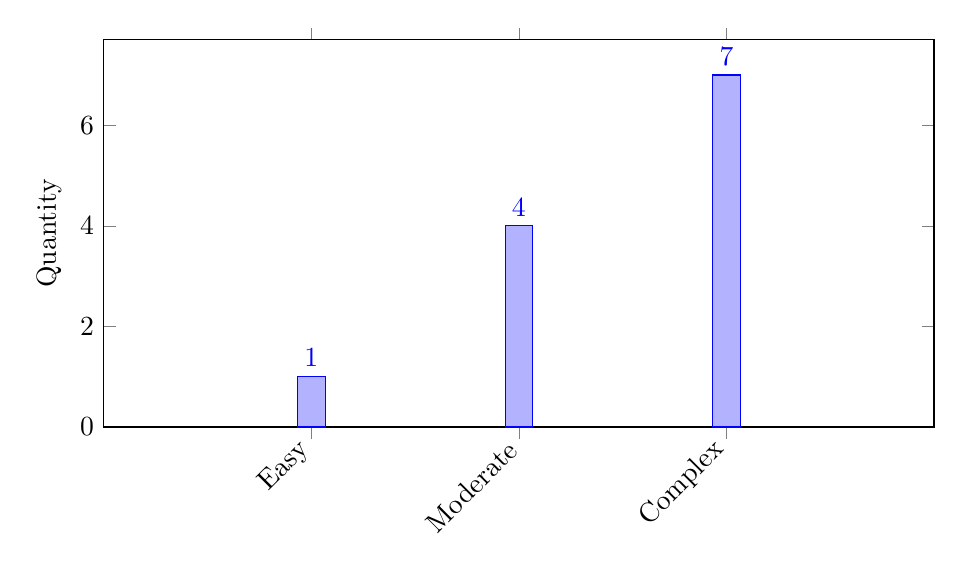
\begin{tikzpicture}
                            \begin{axis}[
                                ybar,
                                width=\textwidth,
                                height=6.5cm,
                                symbolic x coords={Easy, Moderate, Complex},
                                xtick=data,
                                ylabel={Quantity},
                                ymin=0,
                                nodes near coords,
                                enlarge x limits=0.5,
                                x tick label style={rotate=45, anchor=east}
                                ]
                                \addplot coordinates {(Easy, 1) (Moderate, 4) (Complex, 7)};
                            \end{axis}
                        \end{tikzpicture}
                        \subcaption{Perceived difficulty of the monitoring process.}
                        \label{fig:monitoring-process}
                    \end{minipage}
                    \vspace{5mm}
                    \begin{minipage}{0.45\textwidth}
                        \centering
                        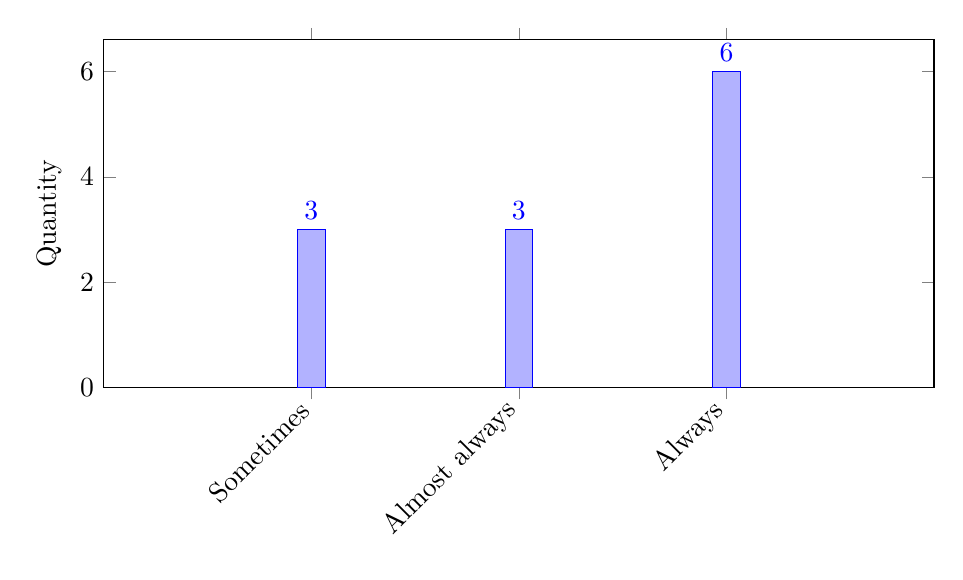
\begin{tikzpicture}
                            \begin{axis}[
                                ybar,
                                width=\textwidth,
                                height=6cm,
                                symbolic x coords={Sometimes, Almost always, Always},
                                xtick=data,
                                ylabel={Quantity},
                                ymin=0,
                                nodes near coords,
                                enlarge x limits=0.5,
                                x tick label style={rotate=45, anchor=east}
                                ]
                                \addplot coordinates {(Sometimes, 3) (Almost always, 3) (Always, 6)};
                            \end{axis}
                        \end{tikzpicture}
                        \subcaption{Frequency of student monitoring.}
                        \label{fig:monitoring-frequency}
                    \end{minipage}
                    \begin{minipage}{0.45\textwidth}
                        \centering
                        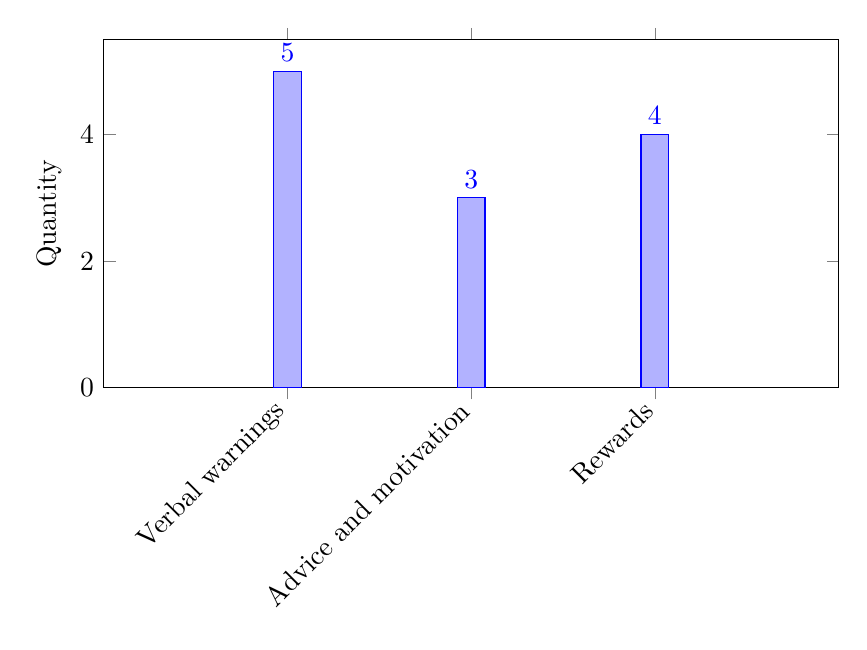
\begin{tikzpicture}
                            \begin{axis}[
                                ybar,
                                height=6cm,
                                width=0.9\textwidth,
                                symbolic x coords={Verbal warnings, Advice and motivation, Rewards},
                                xtick=data,
                                ylabel={Quantity},
                                ymin=0,
                                nodes near coords,
                                enlarge x limits=0.5,
                                x tick label style={rotate=45, anchor=east}
                                ]
                                \addplot coordinates {(Verbal warnings, 5) (Advice and motivation, 3) (Rewards, 4)};
                            \end{axis}
                        \end{tikzpicture}
                        \subcaption{Strategies used to improve concentration.}
                        \label{fig:concentration-strategies}
                    \end{minipage}
                    \caption{Responses from guardians to preliminary questions regarding the monitoring of their elementary school children while completing homework at home.}
                    \label{fig:previous-questions}
                \end{figure}
                
                \paragraph{Tasks Performed by Participating Guardians.}
                The tasks performed by the guardians during the usability evaluation were as follows:
                
                \begin{enumerate}
                    \item Connect the Torddis device to the power source and place it on the desk where the child will sit to complete schoolwork.
                    
                    \item Create a tutor user account in the mobile application.
                    
                    \item Log in to the mobile application.
                    
                    \item Register the child to be monitored.
                    
                    \item Register the Torddis device in the mobile application using the MAC address provided on the device's label.
                    
                    \item Perform facial training for the registered child.
                    
                    \item Enable and/or disable the objects (distractors) to be monitored in the corresponding section of the mobile application.
                    
                    \item Assign a task to the child while being monitored by the Torddis device: colouring a mandala.
                    
                    \item Activate the detection of each distraction parameter in the monitoring section of the mobile application.
                    
                    \item The child remains unsupervised for 6 minutes, in the passive presence of adults (independence condition).
                    
                    \item Enable and/or disable video streaming from the Torddis device.
                    
                    \item Browse the history of monitored distraction parameters for the child.
                    
                    \item View a graphical report displaying the detected distraction parameters for the monitored child.
                \end{enumerate}
                
                \paragraph{System Usability Scale (SUS) Questionnaire Results.}
                The results analysed in this section correspond to the responses to the SUS questionnaire (see Appendix~\ref{Appendix:SUSLikertQuestionary}) provided by the 12 guardians. Based on the collected data, Figure~\ref{fig:sus-questionnaire} shows a mean SUS score of 81.46\%, with a standard deviation of 11.65. According to the adjective ratings (Worst imaginable, Poor, Acceptable, Good, Excellent, Best imaginable) proposed by \cite{Bangor2008AnEmpirical} to qualitatively interpret system usability scores, it is evident that Torddis achieved a “Good” level of usability based on the guardians’ evaluations.
                
                \begin{figure}[!htbp]
                    \centering
                    \begin{tikzpicture}
                        \begin{axis}[
                            scatter/classes={
                                a={mark=*,blue}
                            },
                            width=0.95\linewidth,
                            height=8cm,
                            xlabel={Participant},
                            ylabel={Evaluation Score},
                            ymin=40, ymax=100,
                            xmin=0, xmax=13,
                            xtick={1,2,3,4,5,6,7,8,9,10,11,12},
                            xticklabels={1,2,3,4,5,6,7,8,9,10,11,12},
                            ytick={40,60,80,100},
                            nodes near coords,
                            every node near coord/.append style={font=\footnotesize, /pgf/number format/fixed},
                            legend style={at={(0.5,-0.15)}, anchor=north, legend columns=-1},
                            enlarge x limits=0.05,
                            ]
                            \addplot[
                            scatter,
                            only marks,
                            scatter src=explicit symbolic,
                            visualization depends on=\thisrow{Evaluation} \as \label
                            ] table[meta=class,x=Participant,y=Evaluation] {
                                Participant Evaluation class
                                1 90.00 90.00
                                2 95.00 95.00
                                3 72.50 72.50
                                4 60.00 60.00
                                5 85.00 85.00
                                6 67.50 67.50
                                7 92.50 92.50
                                8 67.50 67.50
                                9 82.50 82.50
                                10 85.00 85.00
                                11 92.50 92.50
                                12 87.50 87.50
                            };
                            
                            % Average line
                            \addplot [
                            color=orange,
                            thick,
                            mark=none
                            ] coordinates {(0,\average) (13,\average)};
                            
                            % Upper standard deviation
                            \addplot [
                            color=orange,
                            thick,
                            dashed,
                            mark=none
                            ] coordinates {(0,\upperlimit) (13,\upperlimit)};
                            
                            % Lower standard deviation
                            \addplot [
                            color=orange,
                            thick,
                            dashed,
                            mark=none
                            ] coordinates {(0,\lowerlimit) (13,\lowerlimit)};
                            
                            \legend{Participant, Mean SUS Score, Std. Deviation}
                        \end{axis}
                    \end{tikzpicture}
                    \caption{Mean and standard deviation of guardians' responses to the SUS questionnaire.}
                    \label{fig:sus-questionnaire}
                \end{figure}
                
                The results of the SUS questionnaire \citep{Brooke1996SUS} reflect a positive perception of the system, with scores emphasizing its ease of use and effectiveness. The consistency in users' responses demonstrates that the interface design and the initial setup processes are properly optimized for users with varying levels of technological experience. This reinforces the robustness of the system as an accessible tool for guardians with different educational backgrounds \citep{Deng2024Does}.
                
                \paragraph{Results of the Open-Ended Questions Questionnaire.}
                At the end of the SUS questionnaire, the guardians answered eight open-ended questions (see Appendix~\ref{Appendix:SUSOpenQuestionarie}) to provide their personal opinions.
                
                The first question was “What is your general opinion about the system?”, to which some guardians responded that it supports students' concentration, while others highlighted its appealing design, as shown in Figure~\ref{fig:AboutTorddis}. The second open-ended question asked was “Did you like the sounds and/or lights used by Torddis?”. Most guardians expressed a favorable opinion, as they believed that light alerts help keep the student awake and were satisfied with the auditory alarms (see Figure~\ref{fig:SoundAndLigth}).
                
                Figures~\ref{fig:AboutTorddis} and~\ref{fig:SoundAndLigth} summarize these opinions.
                
                \begin{figure}[!htbp]
                    \centering
                    \begin{minipage}{0.45\textwidth}
                        \centering
                        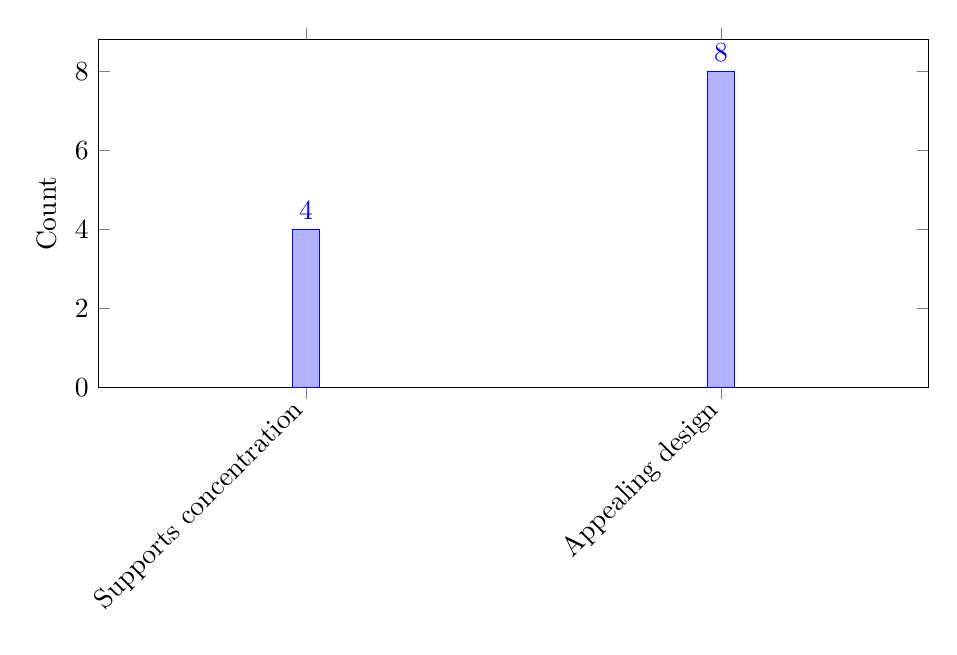
\begin{tikzpicture}
                            \begin{axis}[
                                ybar,
                                width=\textwidth,
                                height=6cm,
                                symbolic x coords={Supports concentration, Appealing design},
                                xtick=data,
                                ylabel={Count},
                                ymin=0,
                                nodes near coords,
                                enlarge x limits=0.5,
                                x tick label style={rotate=45, anchor=east}
                                ]
                                \addplot coordinates {(Supports concentration, 4) (Appealing design, 8)};
                            \end{axis}
                        \end{tikzpicture}
                        \subcaption{General opinion about the Torddis system.}
                        \label{fig:AboutTorddis}
                    \end{minipage}
                    \vspace{5mm}
                    \begin{minipage}{0.45\textwidth}
                        \centering
                        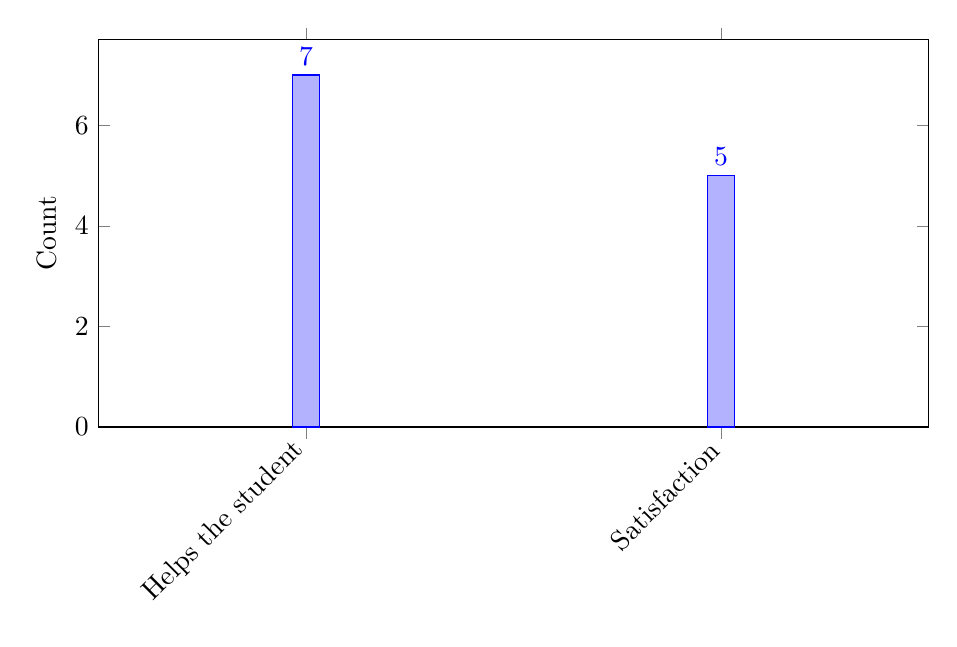
\begin{tikzpicture}
                            \begin{axis}[
                                ybar,
                                width=\textwidth,
                                height=6.5cm,
                                symbolic x coords={Helps the student, Satisfaction},
                                xtick=data,
                                ylabel={Count},
                                ymin=0,
                                nodes near coords,
                                enlarge x limits=0.5,
                                x tick label style={rotate=45, anchor=east}
                                ]
                                \addplot coordinates {(Helps the student, 7) (Satisfaction, 5)};
                            \end{axis}
                        \end{tikzpicture}
                        \subcaption{Auditory and visual alerts of the system.}
                        \label{fig:SoundAndLigth}
                    \end{minipage}
                    \begin{minipage}{0.45\textwidth}
                        \centering
                        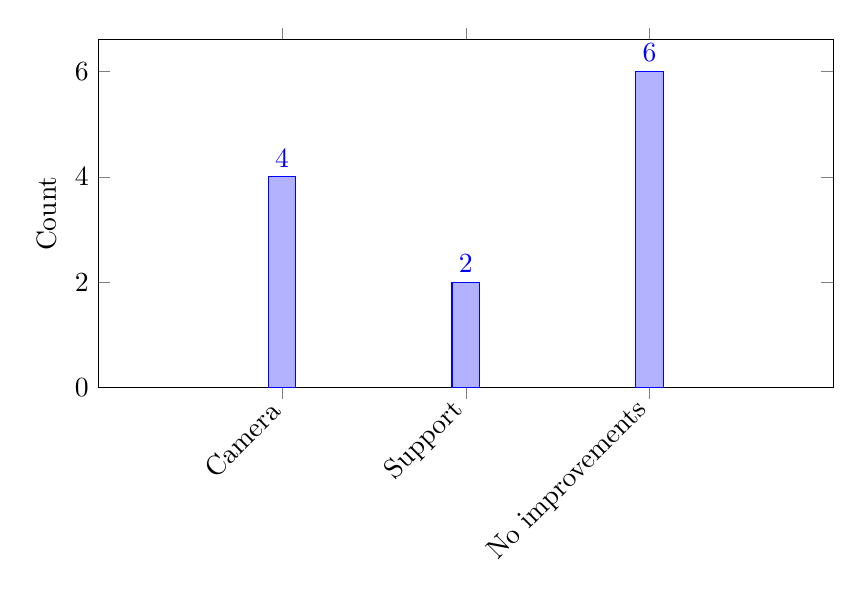
\begin{tikzpicture}
                            \begin{axis}[
                                ybar,
                                height=6cm,
                                width=0.9\textwidth,
                                symbolic x coords={Camera, Support, No improvements},
                                xtick=data,
                                ylabel={Count},
                                ymin=0,
                                nodes near coords,
                                enlarge x limits=0.5,
                                x tick label style={rotate=45, anchor=east}
                                ]
                                \addplot coordinates {(Camera, 4) (Support, 2) (No improvements, 6)};
                            \end{axis}
                        \end{tikzpicture}
                        \subcaption{Suggestions for improving the system.}
                        \label{fig:Improvements}
                    \end{minipage}
                    \begin{minipage}{0.45\textwidth}
                        \centering
                        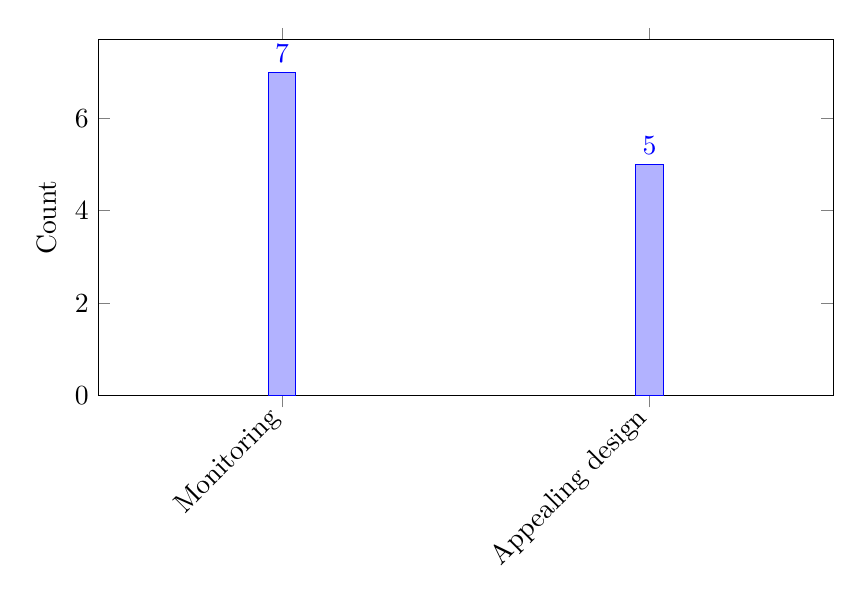
\begin{tikzpicture}
                            \begin{axis}[
                                ybar,
                                height=6.1cm,
                                width=0.9\textwidth,
                                symbolic x coords={Monitoring, Appealing design},
                                xtick=data,
                                ylabel={Count},
                                ymin=0,
                                nodes near coords,
                                enlarge x limits=0.5,
                                x tick label style={rotate=45, anchor=east}
                                ]
                                \addplot coordinates {(Monitoring, 7) (Appealing design, 5)};
                            \end{axis}
                        \end{tikzpicture}
                        \subcaption{Reasons to recommend the system.}
                        \label{fig:ReasonsRecomend}
                    \end{minipage}
                    \caption{Results of guardians’ responses to open-ended questions regarding the monitoring process of their primary school children using Torddis while performing academic tasks at home.}
                    \label{fig:AnswerOfOpenQuestion}
                \end{figure}
                
                Questions 3 (“Do you like the design of the Torddis mobile application? Why?”), 4 (“Is the way the data about your child’s distraction monitoring is displayed in the Torddis mobile app appropriate? Why?”), 5 (“Do you believe this system would help improve your child’s concentration and keep you informed while they do their homework? Why?”), and 7 (“Would you be willing to continue using the Torddis system?”) received entirely positive feedback. The guardians stated that they liked the screen design (graphical interfaces) of the mobile application, praised the organization of historical data and graphical reports, confirmed that the system prototype effectively supports children's concentration by keeping them informed when distractions occur, and expressed their willingness to continue using the Torddis system.
                
                Question 6 aimed to gather information about possible improvements to Torddis. The feedback included the suggestion to use a higher-quality camera and enhance the camera mounting support. However, a high percentage of users indicated that no further improvements were necessary. These results are illustrated in Figure~\ref{fig:Improvements}. Question 8 collected the reasons why guardians would recommend using Torddis for monitoring students during their school-related tasks at home. Figure~\ref{fig:ReasonsRecomend} presents the reasons mentioned by the guardians, highlighting its usefulness in monitoring and its appealing design.
                
                \subsubsection{Recognition Analysis}
                Table~\ref{tab:combined-recognition} presents the average recognition times recorded by Torddis during each test. These average times correspond to the latency in recognizing individuals, facial expressions, drowsiness states, and distracting objects. The number of tests per recognition type ranged from 14 to 32, except for the “Unsuccessful” cases, which occurred in only 1 or 2 trials (depending on the recognition type) where Torddis failed to achieve recognition.
                
                In each trial, the time taken by the system to correctly identify each element was measured in seconds, along with a record of whether the recognition was successful or not.
                
                Although Table~\ref{tab:combined-recognition} includes unsuccessful recognition cases, these were not considered in the main analysis, as the aim was to evaluate response times. Since unsuccessful responses are recorded with a time of 0.00 seconds, their inclusion could bias the results and lead to non-representative statistical values.
                
                \begin{table}[!htbp]
                    \centering
                    \caption{Aggregated recognition results.}
                    \label{tab:combined-recognition}
                    \setlength{\tabcolsep}{3pt}\begin{tabular*}{\linewidth}{@{\extracolsep{\fill}}c *{8}{>{\centering\arraybackslash}p{0.9cm}}@{}}
                        \toprule
                        \multicolumn{1}{c}{\textbf{No.}} & \multicolumn{2}{c}{\textbf{Person Recognition}} & \multicolumn{2}{c}{\textbf{Facial Expression}} & \multicolumn{2}{c}{\textbf{Drowsiness Detection}} & \multicolumn{2}{c}{\textbf{Distracting Objects}}\\
                        \cmidrule(lr){2-3}\cmidrule(lr){4-5}\cmidrule(lr){6-7}\cmidrule(lr){8-9}
                        & \multicolumn{1}{c}{\textbf{Latency}} & \multicolumn{1}{c}{\textbf{Success}} & \multicolumn{1}{c}{\textbf{Latency}} & \multicolumn{1}{c}{\textbf{Success}} & \multicolumn{1}{c}{\textbf{Latency}} & \multicolumn{1}{c}{\textbf{Success}} & \multicolumn{1}{c}{\textbf{Latency}} & \multicolumn{1}{c}{\textbf{Success}} \\
                        \midrule
                        1 & 0.60 & Yes & 1.20 & Yes & 3.50 & Yes & 1.68 & Yes \\
                        2 & 0.57 & Yes & 0.82 & Yes & 2.73 & Yes & 1.68 & Yes \\
                        3 & 0.00 & \textbf{No} & 0.70 & Yes & 0.00 & \textbf{No} & 0.00 & \textbf{No} \\
                        4 & 0.78 & Yes & 1.30 & Yes & 3.68 & Yes & 1.79 & Yes \\
                        5 & 1.02 & Yes & 0.78 & Yes & 2.24 & Yes & 0.00 & \textbf{No} \\
                        6 & 1.20 & Yes & 0.97 & Yes & 2.03 & Yes & 2.05 & Yes \\
                        7 & 0.82 & Yes & 0.87 & Yes & 3.03 & Yes & 1.95 & Yes \\
                        8 & 0.76 & Yes & 1.05 & Yes & 4.09 & Yes & 1.77 & Yes \\
                        9 & 1.20 & Yes & 0.70 & Yes & 3.36 & Yes & 1.91 & Yes \\
                        10 & 0.88 & Yes & 0.00 & \textbf{No} & 2.63 & Yes & 1.98 & Yes \\
                        11 & 0.53 & Yes & 1.23 & Yes & 0.00 & \textbf{No} & 1.73 & Yes \\
                        12 & 0.69 & Yes & 1.99 & Yes & 4.69 & Yes & 4.27 & Yes \\
                        13 & 0.67 & Yes & 1.07 & Yes & 2.97 & Yes & 1.77 & Yes \\
                        14 & 0.82 & Yes & 1.83 & Yes & 3.29 & Yes & 2.69 & Yes \\
                        15 & 0.93 & Yes & 1.68 & Yes & 3.14 & Yes & 2.81 & Yes \\
                        16 & 0.58 & Yes & 1.76 & Yes & 3.45 & Yes & 2.94 & Yes \\
                        \bottomrule
                    \end{tabular*}
                \end{table}
                
                \paragraph{Descriptive Analysis of Recognition Latency Times:}
                Table \ref{tab:latency-stats-transposed} presents the descriptive results of the latency values recorded by Torddis during its operation. This system, designed to be non-intrusive, collects data in real time, which directly influences the quality and distribution of the recorded measurements. The main findings are discussed below:
                
                \begin{table}[!htbp]
                    \centering
                    \caption{Measures of central tendency and dispersion for recognition latency.}
                    \label{tab:latency-stats-transposed}
                    \begin{tabular*}{\linewidth}{@{\extracolsep{\fill}}
                            >{\raggedright\arraybackslash}p{3.5cm}
                            >{\raggedleft\arraybackslash}p{1.8cm}<{\hspace*{6pt}}
                            >{\raggedleft\arraybackslash}p{2cm}<{\hspace*{6pt}}
                            >{\raggedleft\arraybackslash}p{1.8cm}<{\hspace*{6pt}}
                            >{\raggedleft\arraybackslash}p{2cm}<{\hspace*{6pt}}
                            @{}
                        }
                        \toprule
                        \multicolumn{1}{c}{\textbf{Statistic}} & 
                        \multicolumn{1}{c}{\textbf{People}} & 
                        \multicolumn{1}{c}{\textbf{\shortstack{Facial\\Expressions}}} & 
                        \multicolumn{1}{c}{\textbf{\shortstack{Sleep\\Detection}}} & 
                        \multicolumn{1}{c}{\textbf{\shortstack{Distracting\\Objects}}} \\
                        \midrule
                        Number of observations & 15 & 15 & 14 & 14 \\
                        Mean & 0.803 & 1.197 & 3.202 & 2.216 \\
                        Median & 0.780 & 1.070 & 3.215 & 1.930 \\
                        Mode & 0.82 and 1.2 & 0.700 & Amodal & 1.68 and 1.77 \\
                        Standard deviation & 0.213 & 0.431 & 0.699 & 0.732 \\
                        Minimum & 0.530 & 0.700 & 2.030 & 1.680 \\
                        First quartile (Q1) & 0.635 & 0.845 & 2.790 & 1.770 \\
                        Second quartile (Q2) & 0.780 & 1.070 & 3.215 & 1.930 \\
                        Third quartile (Q3) & 0.905 & 1.490 & 3.488 & 2.530 \\
                        Maximum & 1.200 & 1.990 & 4.690 & 4.270 \\
                        \bottomrule
                    \end{tabular*}
                \end{table}
                
                \begin{itemize}
                    \item \textit{Person Recognition:} The low data dispersion, evidenced by the small standard deviation and the closeness among the measures of central tendency (mean, median, and mode), indicates that person detection is consistently achieved across users. This consistency is further supported by the narrow range between the minimum and maximum values, as well as a distribution centered around the quartiles. These findings suggest that Torddis reliably captures clear and stable signals related to human presence without interfering with the environment or participants. The observed uniformity reinforces the robustness of this functionality in non-intrusive contexts.
                    
                    \item \textit{Facial Expression Recognition:} This category exhibits greater variability, as reflected in the standard deviation and in a mode that differs significantly from the mean and median. Although the quartiles indicate some degree of concentration, the range between extreme values is broader than in the previous category. This variability may be attributed to individual differences in facial expressions, as well as to environmental factors such as lighting conditions and capture angle. Although latency values remain within acceptable limits, these conditions can affect recognition accuracy in certain cases, suggesting the need to improve facial recognition algorithms without compromising user comfort.
                    
                    \item \textit{Drowsiness Detection:} Latency values in this category are noticeably higher, with elevated mean and median, as well as a broad range and a distribution without a defined mode (amodal). This situation reflects the inherent complexity of detecting subtle signs of drowsiness through non-intrusive methods. The quartiles indicate considerable dispersion, and the standard deviation reinforces this interpretation. While these results are expected, given that drowsiness signals are less evident, the system could benefit in the future from more specialized techniques or sensors to optimize both the speed and accuracy of detection.
                    
                    \item \textit{Detection and Recognition of Distracting Objects:} The wide range of latency values, combined with a high standard deviation and a bimodal mode, indicates considerable variability in the detection of distracting objects. This can be attributed to the diversity of the physical environment, object movement, or lighting conditions—typical variables in uncontrolled settings. Nevertheless, the distribution of the quartiles and the relative proximity between the mean and median suggest that, although complete uniformity is not achieved, the system is capable of recognizing distracting objects in most cases, demonstrating reasonable performance in dynamic and real-world scenarios.
                \end{itemize}
                
                \paragraph{Correlation Between Latency Times:} 
                To compute the correlation matrix, missing values (to complete a total of 16 valid entries) were replaced with the mean latency corresponding to each category. The correlation matrix of latency times for the recognition of people, distracting objects, facial expressions, and drowsiness detection is presented in Table~\ref{tab:correlation-latency}. This matrix allows for the examination of linear relationships between the latencies of the different system modules: \textit{person detection}, \textit{facial expression recognition}, \textit{drowsiness detection}, and \textit{distracting object identification}. It was constructed using Pearson's correlation coefficient (\(r\)), which quantifies the strength and direction of the linear association between pairs of numerical variables.
                
                \begin{table}[!htbp]
                    \centering
                    \caption{Correlation matrix of recognition module latencies.}
                    \label{tab:correlation-latency}
                    \begin{tabular*}{\linewidth}{@{\extracolsep{\fill}}
                            >{\raggedright\arraybackslash}p{3.5cm}
                            >{\raggedleft\arraybackslash}p{1.8cm}<{\hspace*{8pt}}
                            >{\raggedleft\arraybackslash}p{2.2cm}<{\hspace*{8pt}}
                            >{\raggedleft\arraybackslash}p{1.8cm}<{\hspace*{8pt}}
                            >{\raggedleft\arraybackslash}p{1.8cm}<{\hspace*{8pt}}
                            @{}
                        }
                        \toprule
                        & \multicolumn{1}{c}{\textbf{People}} & \multicolumn{1}{c}{\textbf{\shortstack{Facial\\Expressions}}} & \multicolumn{1}{c}{\textbf{Drowsiness}} & \multicolumn{1}{c}{\textbf{Objects}} \\
                        
                        \midrule
                        \textbf{People} & 1.000 & -0.332 & -0.426 & -0.031 \\
                        
                        \textbf{Facial Expressions} & -0.332 & 1.000 & 0.521 & 0.744 \\
                        
                        \textbf{Drowsiness} & -0.426 & 0.521 & 1.000 & 0.476 \\
                        
                        \textbf{Objects} & -0.031 & 0.744 & 0.476 & 1.000 \\
                        \bottomrule
                    \end{tabular*}
                \end{table}		
                
                The analysis reveals a strong positive correlation between the latencies of the \textit{facial expressions} and \textit{distracting objects} modules (\(r = 0.744\)), suggesting a high degree of interdependence between these processes. This behavior may be attributed to the combined use of deep visual analysis techniques, which involve intensive processing of facial images, or to a shared architecture in the computational implementation that simultaneously evaluates multiple features within the same regions of interest.
                
                A moderate positive correlation is also observed between \textit{facial expressions} and \textit{drowsiness} detection (\(r = 0.521\)), and between \textit{drowsiness} and \textit{distracting objects} (\(r = 0.476\)). These coefficients indicate that an increase in latency in one of these modules tends to be associated with proportional increases in the others, which could be linked to the shared computational resource load, such as the use of the graphics coprocessor or common inference libraries.
                
                In contrast, latency in the \textit{person detection} module exhibits moderate negative correlations with both \textit{facial expression recognition} (\(r = {-}0.332\)) and \textit{drowsiness detection} (\(r = {-}0.426\)). This pattern suggests a possible competition for resources among these modules or a prioritization in the execution flow that reduces latency in one process at the expense of increasing it in another.
                
                Finally, the near-zero correlation between latency in the \textit{person recognition} and \textit{distracting objects} modules (\(r = -0.031\)) indicates that these modules operate statistically independently in terms of execution time. Such functional independence may be advantageous for optimizing parallel or segmented execution in future iterations of the system.
                
                In summary, this quantitative analysis enables the identification of significant relationships between system components, revealing both synergies and potential performance conflicts, which are essential for enhancing architectural design and operational efficiency in mobile environments.
                
                
                \subsection{Statistical Analysis of Guardians' Responses}
                \label{sec:stats-analysis}

                Statistical analysis plays a fundamental role in the understanding and evaluation of systems such as Torddis, enabling the transformation of collected data into robust evidence that supports the study’s conclusions. This approach is essential for identifying patterns, relationships, and significant differences among the evaluated variables, ensuring that the results accurately reflect the dynamics observed during the use of the device.
                
                Through descriptive and analytical statistical methods, a rigorous validation of the findings is ensured, highlighting key aspects of the system such as its acceptance by users, its effectiveness in enhancing self-regulation, and its pedagogical impact. The application of appropriate statistical tools not only reinforces the reliability of the results but also provides a solid foundation for future improvements and implementations of the system in diverse educational contexts.
                
                \subsubsection{Descriptive Statistics}
                This section presents and analyzes the descriptive statistics obtained from the collected data. These statistics play a crucial role in understanding the behavior of the evaluated variables and their impact on the acceptance and effectiveness of the system.
                
                Table \ref{table:DescriptiveStatistics} shows measures of central tendency, such as the mean and median, which allow for the identification of general patterns among tutors and students regarding the Torddis system. For instance, the average daily time devoted by tutors to supervising school tasks is 2 hours, indicating active but limited participation due to their time constraints caused by everyday responsibilities. The responses to the statements related to the perception and use of the device (Statements (1) to (7), see Appendix \ref{Appendix:LikertEffectivity}) reveal consistently high average values (ranging from 3.58 to 4.42 on a 5-point Likert scale), suggesting a general acceptance of the system.
                
                \begin{table}[!htbp]
                    \centering
                    \caption{Descriptive statistics on supervision time and the usage and effectiveness of the developed device.}
                    \setlength{\tabcolsep}{3pt}\begin{tabular*}{\linewidth}{@{\extracolsep{\fill}}>{\raggedright\arraybackslash}p{2.6cm} *{8}{>{\raggedleft\arraybackslash}p{0.85cm}<{\hspace*{3pt}}}@{}}
                        \toprule
                        \multicolumn{1}{c}{\textbf{Statistic}} & \multicolumn{1}{c}{\textbf{\shortstack{Superv.\\Time}}} & \multicolumn{1}{c}{\textbf{(1)}} & \multicolumn{1}{c}{\textbf{(2)}} & \multicolumn{1}{c}{\textbf{(3)}} & \multicolumn{1}{c}{\textbf{(4)}} & \multicolumn{1}{c}{\textbf{(5)}} & \multicolumn{1}{c}{\textbf{(6)}} & \multicolumn{1}{c}{\textbf{(7)}} \\
                        \midrule
                        Mean & 2.00 & 4.42 & 4.42 & 2.67 & 3.58 & 4.00 & 4.42 & 4.42 \\
                        Median & 2.00 & 5.00 & 4.00 & 3.00 & 4.00 & 4.00 & 5.00 & 5.00 \\
                        Standard Deviation & 0.69 & 0.90 & 0.67 & 0.98 & 0.90 & 0.85 & 0.79 & 0.79 \\
                        Minimum & 1.00 & 3.00 & 3.00 & 1.00 & 2.00 & 3.00 & 3.00 & 3.00 \\
                        Maximum & 3.00 & 5.00 & 5.00 & 4.00 & 5.00 & 5.00 & 5.00 & 5.00 \\
                        \bottomrule
                    \end{tabular*}
                    \label{table:DescriptiveStatistics}
                    \vspace{0.3em} % Space between table and note
                    \parbox{0.85\textwidth}{\footnotesize
                        Items (n) with $n=1\ldots7$ correspond to the seven statements evaluated on a 5-point Likert scale related to the prototype’s effectiveness (see Appendix \ref{Appendix:LikertEffectivity}, Table \ref{tab:EffectivityQuestions}). \textit{Supervision time} represents the number of daily hours that tutors dedicate to supervising their children’s schoolwork.
                    }
                \end{table}
                
                On the other hand, dispersion indicators, such as the standard deviation, provide insight into the variability of the responses. The standard deviation for the statements (ranging from 0.67 to 0.98) indicates that participants' perceptions were relatively homogeneous, which reinforces the consistency in the user experience of the device. However, the greater variability in \textit{Statement (3)} suggests that some students may have perceived the device as more intrusive, which could necessitate design adjustments.
                
                Likewise, the minimum and maximum values reveal possible differences in participants’ experiences, highlighting areas that may require improvement. For instance, while some tutors reported dedicating only one hour to supervision, others reached up to three hours, which could influence the responses related to the system’s effectiveness.
                
                These results make it possible to identify not only the general level of acceptance of the system but also specific areas that could benefit from targeted future interventions. Taken together, the descriptive statistics provide a foundation for validating the device’s design and supporting the discussion regarding its pedagogical and practical potential.
                
                \subsubsection{Normality Analysis of the Data}
                To determine whether the numerical variables follow a normal distribution, two complementary tests were applied: the Shapiro–Wilk (SW) test and the Kolmogorov–Smirnov (KS) test \citep{Correa2025Simulation}. The SW test is highly sensitive to deviations from normality and is particularly suitable for small sample sizes, whereas the KS test compares the empirical distribution of the data with a theoretical distribution (in this case, the normal distribution) and is more robust in the presence of heterogeneous variance or larger sample sizes \citep{Kobayashi2025Testing}. Both tests were employed to ensure a comprehensive analysis by evaluating different aspects of normality in the data.
                
                The results presented in Table \ref{tab:NormalityTest} show that the SW and KS tests do not always produce consistent conclusions, as they assess different properties of the normality assumption \citep{Correa2025Simulation}. Therefore, the results of both tests were interpreted in a complementary manner to achieve a more robust evaluation of the normality of the dataset.
                
                \begin{table}[!htbp]
                    \centering
                    \caption{Results of the normality analysis for tutors' responses to the effectiveness questions}
                    \begin{tabular*}{\linewidth}{@{\extracolsep{\fill}}
                            >{\raggedright\arraybackslash}p{3.5cm}
                            >{\raggedleft\arraybackslash}p{1.8cm}<{\hspace*{6pt}}
                            >{\centering\arraybackslash}p{2cm}
                            >{\raggedleft\arraybackslash}p{1.8cm}<{\hspace*{6pt}}
                            >{\centering\arraybackslash}p{2cm}
                            @{}}
                        \toprule
                        \multicolumn{1}{c}{\textbf{Variable}} & \multicolumn{1}{c}{\textbf{\shortstack{SW\\\textit{p}-value}}} & \multicolumn{1}{c}{\textbf{\shortstack{SW\\Conclusion}}} & \multicolumn{1}{c}{\textbf{\shortstack{KS\\\textit{p}-value}}} & \multicolumn{1}{c}{\textbf{\shortstack{KS\\Conclusion}}} \\
                        \midrule
                        Tutor's Age & 0.2277 & \(\checkmark\) & 0.9289 & \(\checkmark\) \\
                        Supervision Time & 0.0119 & \(\times\) & 0.1885 & \(\checkmark\) \\
                        Student's Age & 0.1736 & \(\checkmark\) & 0.6257 & \(\checkmark\) \\
                        Statement (1) & 0.0016 & \(\times\) & 0.0775 & \(\checkmark\) \\
                        Statement (2) & 0.0063 & \(\times\) & 0.2562 & \(\checkmark\) \\
                        Statement (3) & 0.0528 & \(\checkmark\) & 0.1898 & \(\checkmark\) \\
                        Statement (4) & 0.0598 & \(\checkmark\) & 0.2081 & \(\checkmark\) \\
                        Statement (5) & 0.0199 & \(\times\) & 0.3779 & \(\checkmark\) \\
                        Statement (6) & 0.0016 & \(\times\) & 0.0775 & \(\checkmark\) \\
                        Statement (7) & 0.0016 & \(\times\) & 0.0775 & \(\checkmark\) \\
                        \bottomrule
                    \end{tabular*}
                    \label{tab:NormalityTest}
                    \vspace{0.3em} % Spacing between table and caption
                    \parbox{0.75\textwidth}{\footnotesize
                        \(\times\): Does not follow a normal distribution. \(\checkmark\): Follows a normal distribution.\\
                        SW = Shapiro–Wilk. KS = Kolmogorov–Smirnov.
                    }
                \end{table}
                
                The \textit{p-value} shown in Table~\ref{tab:NormalityTest} for both tests indicates whether the null hypothesis is accepted or rejected; that is, whether the variables follow a normal distribution or not. The columns \textit{SW Conclusion} and \textit{KS Conclusion} display the results of the hypothesis testing (H\textsubscript{0}: The variable follows a normal distribution. H\textsubscript{1}: The variable does not follow a normal distribution).
                
                While the KS test indicates that all variables follow a normal distribution, the SW test suggests that some variables conform to normality, whereas others do not. To ensure the validity of subsequent analyses, appropriate statistical tests were selected based on these results. Nevertheless, the Pearson correlation coefficient test was applied to all variables.
                
                \subsubsection{Correlation between Statement (5) and the Other Variables}
                Pearson correlation tests were employed to explore significant relationships and differences among the variables under study and their corresponding factors. Considering all variables as normally distributed, the Pearson correlation analysis enabled the identification of relationships between the variable \textit{``Statement (5): \textit{After discontinuing use of the device, the student demonstrated improvement in self-regulation and concentration while completing homework at home}''} and the remaining numerical variables. The correlations observed were statistically significant in several cases, highlighting important patterns regarding the impact of the device, as shown in Table~\ref{table:Pearson-Correlation}.
                
                \begin{table}[!htbp]
                    \centering
                    \caption{Correlations between Statement (5) and the Other Variables}
                    \begin{tabular*}{\linewidth}{@{\extracolsep{\fill}}
                            >{\raggedright\arraybackslash}p{4cm}
                            >{\raggedleft\arraybackslash}p{3cm}<{\hspace*{8pt}}
                            >{\raggedleft\arraybackslash}p{2cm}<{\hspace*{8pt}}
                            >{\centering\arraybackslash}p{2.8cm}
                            @{}}
                        \toprule
                        \multicolumn{1}{c}{\textbf{Variable}} & \multicolumn{1}{c}{\textbf{\shortstack{Correlation with\\Statement (5)}}} & \multicolumn{1}{c}{\textbf{\textit{p}-value}} & \multicolumn{1}{c}{\textbf{\shortstack{Type of\\Relationship}}} \\
                        \midrule
                        Age of the tutor$^{sw}$ & -0.2725 & 0.3916 & \(\bigtriangleup\) \\ % Weak
                        Supervision time & -0.1841 & 0.5668 & \(\bigtriangleup\) \\ % Weak
                        Age of the student$^{sw}$ & -0.1407 & 0.6627 & \(\bigtriangleup\) \\ % Weak
                        Statement (1) & 0.7762 & 0.0030 & \(\bigstar\) \\ % Very Strong
                        Statement (2) & 0.5669 & 0.0546 & \(\checkmark\) \\ % Strong
                        Statement (3)$^{sw}$ & 0.7500 & 0.0050 & \(\bigstar\) \\ % Very Strong
                        Statement (4)$^{sw}$ & 0.8165 & 0.0012 & \(\bigstar\) \\ % Very Strong
                        Statement (6) & 0.7762 & 0.0030 & \(\bigstar\) \\ % Very Strong
                        Statement (7) & 0.7762 & 0.0030 & \(\bigstar\) \\ % Very Strong
                        \bottomrule
                    \end{tabular*}
                    \label{table:Pearson-Correlation}
                    \vspace{0.3em} % Space between the table and the footnote
                    \parbox{0.75\textwidth}{\footnotesize
                        $^{sw}$ Normal variables according to the Shapiro-Wilk test.\\
                        \(\bigtriangleup\): Weak. \(\checkmark\): Strong. \(\bigstar\): Very Strong.
                    }
                \end{table}
                
                Firstly, the variables associated with the following statements—\textbf{Statement (1)}: \textit{The device was perceived by the student as appealing}, \textbf{Statement (3)}: \textit{The student did not perceive the presence of the device as intrusive}, \textbf{Statement (4)}: \textit{The device was used throughout the effective time devoted to performing school tasks}, \textbf{Statement (6)}: \textit{Although the device usage time was short, it is expected to significantly contribute to task completion and the academic performance of the student}, and \textbf{Statement (7)}: \textit{You would be willing to continue using the device}—showed \textit{very strong} positive correlations with \textit{Statement (5)}, with values ranging from 0.7500 to 0.8165. In addition, \textbf{Statement (2)}: \textit{The mobile application accurately recorded the events that occurred}, yielded a strong correlation (p-value = 0.5669).
                
                Although age is often regarded as an indicator of greater responsibility \citep{Moss2018Why}, in this study, the variables \textit{Age of the tutor} and \textit{Age of the student} exhibited weak and non-significant correlations, with values of \textbf{-0.2725} and \textbf{-0.1407}, respectively. These findings suggest that the perceived effectiveness of the device is not influenced by the age of either tutors or students. This result highlights the versatility of the system, demonstrating its applicability across diverse demographic groups without being constrained by age-related factors.
                
                Finally, the results underscore that characteristics directly related to device usage—such as its design and operational effectiveness—have a greater impact on improving self-regulation than demographic factors. This provides strong evidence that user-centered design is a key strategy in the development of technology-based educational systems.
                
                \subsubsection{ANOVA Analysis}
                The ANOVA analysis conducted on the variables related to \textit{Statement (5)} revealed significant differences in several statements associated with the effectiveness of the Torddis device, while other variables did not exhibit notable differences. The results presented in Table~\ref{table:ANOVA-Results} have important implications for assessing the system's impact across different dimensions.
                
                \begin{table}[!htbp]
                    \centering
                    \caption{ANOVA analysis results}
                    \begin{tabular*}{\linewidth}{@{\extracolsep{\fill}}
                            >{\raggedright\arraybackslash}p{4.5cm}
                            >{\raggedleft\arraybackslash}p{2.5cm}<{\hspace*{8pt}}
                            >{\raggedleft\arraybackslash}p{2.5cm}<{\hspace*{8pt}}
                            >{\centering\arraybackslash}p{2.5cm}
                            @{}}
                        \toprule
                        \multicolumn{1}{c}{\textbf{Variable}} & \multicolumn{1}{c}{\textbf{\textit{F}-Statistic}} & \multicolumn{1}{c}{\textbf{\textit{p}-value}} & \multicolumn{1}{c}{\textbf{Conclusion}} \\
                        \midrule
                        Tutor's Age$^{sw}$ & 0.8162 & 0.4723 & \(\times\) \\ % No significant differences
                        Supervision Time & 0.2411 & 0.7907 & \(\times\) \\ % No significant differences
                        Student's Age$^{sw}$ & 1.6419 & 0.2467 & \(\times\) \\ % No significant differences
                        Statement (1) & 11.0625 & 0.0038 & \(\bigstar\) \\ % Highly significant difference
                        Statement (2) & 2.9118 & 0.1059 & \textit{NS} \\ % Not significant
                        Statement (3)$^{sw}$ & 5.7857 & 0.0242 & \(\checkmark\) \\ % Significant difference
                        Statement (4)$^{sw}$ & 10.6875 & 0.0042 & \(\bigstar\) \\ % Highly significant difference
                        Statement (6) & 11.0625 & 0.0038 & \(\bigstar\) \\ % Highly significant difference
                        Statement (7) & 11.0625 & 0.0038 & \(\bigstar\) \\ % Highly significant difference
                        \bottomrule
                    \end{tabular*}
                    \label{table:ANOVA-Results}
                    \vspace{0.3em} % Spacing between table and footnote
                    \parbox{0.75\textwidth}{\footnotesize
                        $^{sw}$ Variables following a normal distribution according to the Shapiro–Wilk test.\\
                        \(\times\): No significant differences. \textit{NS}: Not significant. \(\checkmark\): Significant difference. \(\bigstar\): Highly significant difference.
                    }
                \end{table}
                
                Statement (1), which assesses the perceived attractiveness of the device, along with Statements (4), (6), and (7), which address aspects related to the use of the device, exhibited \textit{highly significant differences}, thereby reinforcing the system’s versatility and effectiveness. Statement (3), related to the discretion of the device, presented \textit{p}-values below 0.05, indicating statistically significant differences among the evaluated groups. This supports the notion that the device’s design has a differential impact on its acceptance and perception, potentially influenced by contextual factors such as the age or environment of the learner.
                
                On the other hand, variables such as the tutor’s age, the student’s age, and supervision time did not show statistically significant differences (\textit{p}>0.05), suggesting that the impact of the Torddis system is not conditioned by these demographic variables. This further reinforces the notion that the system is inclusive and adaptable to a wide range of user profiles.
                
                \subsubsection{Post Hoc Tests for Variables with Significant Differences}
                Post Hoc tests \citep{Ogrodniczek2025Comparative} were conducted to identify the specific groups in which statistically significant differences were observed in the ANOVA results presented in Table \ref{table:ANOVA-Results}:
                
                \begin{itemize}
                    \item \textbf{Statement (1):} The results shown in Table \ref{table:posthoc_1} revealed statistically significant differences between groups 3 and 4 (\textit{p}=0.0079), and between groups 3 and 5 (\textit{p}=0.0049). This indicates that the attractiveness of the device is perceived differently across some user subgroups, which may be related to individual or contextual preferences.
                    
                    \begin{table}[!htbp]
                        \centering
                        \caption{Post hoc tests for 'Statement (1)'.}
                        \begin{tabular*}{\linewidth}{@{\extracolsep{\fill}}>{\centering\arraybackslash}p{1.3cm} >{\centering\arraybackslash}p{1.3cm} >{\raggedleft\arraybackslash}p{1.8cm}<{\hspace*{4pt}} >{\raggedleft\arraybackslash}p{1.4cm}<{\hspace*{4pt}} >{\raggedleft\arraybackslash}p{1.6cm}<{\hspace*{4pt}} >{\raggedleft\arraybackslash}p{1.6cm}<{\hspace*{4pt}} >{\centering\arraybackslash}p{1.3cm}@{}}
                            \toprule
                            \textbf{Group 1} & \textbf{Group 2} & \textbf{\shortstack{Mean\\Difference}} & \textbf{\textit{p}-value} & \textbf{\shortstack{Lower\\Bound}} & \textbf{\shortstack{Upper\\Bound}} & \textbf{Rejected} \\
                            \midrule
                            3 & 4 & 1.3333 & 0.0079 & 0.4027 & 2.264 & Yes \\
                            3 & 5 & 1.6667 & 0.0049 & 0.5920 & 2.7413 & Yes \\
                            4 & 5 & 0.3333 & 0.5951 & -0.5973 & 1.264 & No \\
                            \bottomrule
                        \end{tabular*}
                        \label{table:posthoc_1}
                    \end{table}
                    
                    \item \textbf{Statement (3):} Although this statement exhibited statistically significant differences in the ANOVA analysis, the Post Hoc tests identified significance only between groups 3 and 5 (\textit{p} = 0.0194), as shown in Table \ref{table:posthoc_3}. This suggests that not all subgroups perceive the discretion of the device in the same manner.
                    
                    \begin{table}[!htbp]
                        \centering
                        \caption{Post hoc tests for 'Statement (3)'.}
                        \begin{tabular*}{\linewidth}{@{\extracolsep{\fill}}>{\centering\arraybackslash}p{1.3cm} >{\centering\arraybackslash}p{1.3cm} >{\raggedleft\arraybackslash}p{1.8cm}<{\hspace*{4pt}} >{\raggedleft\arraybackslash}p{1.4cm}<{\hspace*{4pt}} >{\raggedleft\arraybackslash}p{1.6cm}<{\hspace*{4pt}} >{\raggedleft\arraybackslash}p{1.6cm}<{\hspace*{4pt}} >{\centering\arraybackslash}p{1.3cm}@{}}
                            \toprule
                            \textbf{Group 1} & \textbf{Group 2} & \textbf{\shortstack{Mean\\Difference}} & \textbf{\textit{p}-value} & \textbf{\shortstack{Lower\\Bound}} & \textbf{\shortstack{Upper\\Bound}} & \textbf{Reject H$_0$} \\
                            \midrule
                            3 & 4 & 1.0000 & 0.1769 & -0.4216 & 2.4216 & No \\
                            3 & 5 & 2.0000 & 0.0194 & 0.3585 & 3.6415 & Yes \\
                            4 & 5 & 1.0000 & 0.1769 & -0.4216 & 2.4216 & No \\
                            \bottomrule
                        \end{tabular*}
                        \label{table:posthoc_3}
                    \end{table}
                    
                    \item \textbf{Statement (4):} Statistically significant differences were observed between Groups 3 and 4 (\textit{p}=0.0176), and between Groups 3 and 5 (\textit{p}=0.0038), as shown in Table \ref{table:posthoc_4}. This indicates that the effective use of the device varies depending on the group, which may be related to factors such as the level of supervision or environmental conditions.
                    
                    \begin{table}[!htbp]
                        \centering
                        \caption{Post hoc tests for 'Statement (4)'.}
                        \begin{tabular*}{\linewidth}{@{\extracolsep{\fill}}>{\centering\arraybackslash}p{1.3cm} >{\centering\arraybackslash}p{1.3cm} >{\raggedleft\arraybackslash}p{1.8cm}<{\hspace*{4pt}} >{\raggedleft\arraybackslash}p{1.4cm}<{\hspace*{4pt}} >{\raggedleft\arraybackslash}p{1.6cm}<{\hspace*{4pt}} >{\raggedleft\arraybackslash}p{1.6cm}<{\hspace*{4pt}} >{\centering\arraybackslash}p{1.3cm}@{}}
                            \toprule
                            \textbf{Group 1} & \textbf{Group 2} & \textbf{\shortstack{Mean\\Difference}} & \textbf{\textit{p}-value} & \textbf{\shortstack{Lower\\Bound}} & \textbf{\shortstack{Upper\\Bound}} & \textbf{Rejected} \\
                            \midrule
                            3 & 4 & 1.3333 & 0.0176 & 0.2587 & 2.408 & Yes \\
                            3 & 5 & 2.0000 & 0.0038 & 0.7591 & 3.2409 & Yes \\
                            4 & 5 & 0.6667 & 0.2461 & -0.408 & 1.7413 & No \\
                            \bottomrule
                        \end{tabular*}
                        \label{table:posthoc_4}
                    \end{table}
                    
                    \item \textbf{Statements (6) and (7):} The Post Hoc tests revealed patterns similar to those observed in Statement (1), showing significant differences between Groups 3 and 4, as well as between Groups 3 and 5. These findings support the positive perception regarding the device’s impact on self-regulation and the intention to continue its use.
                    
                    \begin{table}[!htbp]
                        \centering
                        \caption{Post hoc tests for 'Statement (6) and (7)'}
                        \begin{tabular*}{\linewidth}{@{\extracolsep{\fill}}>{\centering\arraybackslash}p{1.3cm} >{\centering\arraybackslash}p{1.3cm} >{\raggedleft\arraybackslash}p{1.8cm}<{\hspace*{4pt}} >{\raggedleft\arraybackslash}p{1.4cm}<{\hspace*{4pt}} >{\raggedleft\arraybackslash}p{1.6cm}<{\hspace*{4pt}} >{\raggedleft\arraybackslash}p{1.6cm}<{\hspace*{4pt}} >{\centering\arraybackslash}p{1.3cm}@{}}
                            \toprule
                            \textbf{Group 1} & \textbf{Group 2} & \textbf{\shortstack{Mean\\Difference}} & \textbf{\textit{p}-value} & \textbf{\shortstack{Lower\\Bound}} & \textbf{\shortstack{Upper\\Bound}} & \textbf{Reject} \\
                            \midrule
                            3 & 4 & 1.3333 & 0.0079 & 0.4027 & 2.264 & Yes \\
                            3 & 5 & 1.6667 & 0.0049 & 0.5920 & 2.7413 & Yes \\
                            4 & 5 & 0.3333 & 0.5951 & -0.5973 & 1.264 & No \\
                            \bottomrule
                        \end{tabular*}
                        \label{table:posthoc_6y7}
                    \end{table}
                    
                \end{itemize}
                
                These results highlight that Torddis is an effective and versatile tool, whose impact may vary depending on contextual factors such as the environment and user preferences. The identification of significant differences among specific groups underscores the need to tailor certain aspects of the device’s design and implementation in order to maximize its effectiveness across diverse educational settings.
                
                Overall, the statements related to the use and acceptance of the device proved to be relevant in the evaluation of Torddis, while demographic and contextual variables did not significantly condition its effectiveness. This reinforces the system’s robustness and its general applicability in a wide range of user profiles and learning environments.
                
                \subsubsection{Tests for Variables That Do Not Follow a Normal Distribution According to the SW Test}
                For the variables \textit{Supervision time}, \textit{Statement (1)}, \textit{Statement (2)}, \textit{Statement (6)}, and \textit{Statement (7)}, whose p-value was less than 0.05 in the Shapiro-Wilk test, non-parametric tests were applied \citep{Smeeton2025Applied}. In this case, Spearman’s rank correlation coefficient \citep{Yu2024Robust} was used to analyze relationships between these variables, and the Kruskal-Wallis (KW) test \citep{Jamil2024Influence} was applied to both categorical variables and numerical variables that did not follow a normal distribution, in order to assess significant differences among groups.
                
                Table \ref{table:kruskal-spearman-results} presents the results from applying Spearman’s correlation coefficient and the KW test, showing the observed differences among the variables in relation to \textit{Statement (5)}, which assesses the perceived improvement in self-regulation and concentration of the tutee after using the Torddis system. A detailed analysis of the meaning of these results is provided below.
                
                \begin{table}[!htbp]
                    \centering
                    \caption{Results of Kruskal-Wallis and Spearman correlation Tests with respect to Statement (5)}
                    \begin{tabular*}{\linewidth}{@{\extracolsep{\fill}}
                            >{\raggedright\arraybackslash}p{3.5cm}
                            >{\raggedleft\arraybackslash}p{1.7cm}<{\hspace*{4pt}}
                            >{\raggedleft\arraybackslash}p{1.7cm}<{\hspace*{4pt}}
                            >{\raggedleft\arraybackslash}p{1.7cm}<{\hspace*{4pt}}
                            >{\raggedleft\arraybackslash}p{1.5cm}<{\hspace*{4pt}}
                            >{\centering\arraybackslash}p{1.7cm}
                            @{}}
                        \toprule
                        \multicolumn{1}{c}{\textbf{Variable}} & \multicolumn{1}{c}{\textbf{\shortstack{Spearman\\\textit{r}}}} & \multicolumn{1}{c}{\textbf{\shortstack{Spearman\\\textit{p}}}} & \multicolumn{1}{c}{\textbf{\shortstack{KW\\Statistic}}} & \multicolumn{1}{c}{\textbf{\shortstack{KW\\\textit{p}}}} & \multicolumn{1}{c}{\textbf{Conclusions}} \\
                        \midrule
                        Tutor's Education Level & 0.0000 & 1.0000 & 0.0000 & 1.0000 & \(\times\) \(\emptyset\) \\
                        Tutor's Gender & -0.2500 & 0.4332 & 0.6875 & 0.4070 & \(\vartriangle\) \(\emptyset\) \\
                        Area of Residence & 0.0000 & 1.0000 & 0.0000 & 1.0000 & \(\times\) \(\emptyset\) \\
                        Occupation & 0.0000 & 1.0000 & 0.0000 & 1.0000 & \(\times\) \(\emptyset\) \\
                        Type of Internet Signal & -0.2500 & 0.4332 & 0.6875 & 0.4070 & \(\vartriangle\) \(\emptyset\) \\
                        Supervision Time & 0.1925 & 0.5490 & 0.8730 & 0.6463 & \(\vartriangle\) \(\triangleleft\) \\
                        Statement (1) & 0.7698 & 0.0034 & 6.6349 & 0.0362 & \(\bigstar\) \(\checkmark\) \\
                        Statement (2) & 0.5508 & 0.0635 & 3.6056 & 0.1648 & \(\triangle\) \(\times\) \\
                        Statement (6) & 0.7698 & 0.0034 & 6.6349 & 0.0362 & \(\bigstar\) \(\checkmark\) \\
                        Statement (7) & 0.7698 & 0.0034 & 6.6349 & 0.0362 & \(\bigstar\) \(\checkmark\) \\
                        \bottomrule
                    \end{tabular*}
                    \label{table:kruskal-spearman-results}
                    \parbox{\textwidth}{\footnotesize 
                        \(\times\): No correlation. \(\vartriangle\): Weak correlation. \(\triangle\): Moderate correlation. \(\bigstar\): Strong correlation. \(\emptyset\): No significant difference. \(\triangleleft\): No significant effect. \(\checkmark\): Significant difference.
                    }
                \end{table}
                
                Categorical variables such as \textit{Tutor's Education Level}, \textit{Tutor's Gender}, \textit{Area of Residence}, \textit{Occupation}, and \textit{Type of Internet Signal} did not exhibit significant differences according to the Kruskal-Wallis test (\(\emptyset\)), indicating that these characteristics do not significantly influence the perceived effectiveness of the device. Furthermore, their Spearman correlation coefficients ranged from -0.2500 to 0.0000, reinforcing the absence of significant relationships with the response variable.
                
                In contrast, \textit{Statement (1)}, \textit{Statement (6)}, and \textit{Statement (7)} showed significant differences (\(\checkmark\)) and strong correlations (\(\bigstar\)) with \textit{Statement (5)}. These results suggest that positive perceptions regarding the device's usefulness, willingness to continue using it, and its impact on completing academic tasks are directly related to the perceived improvement in the tutee’s self-regulation and concentration. This finding underscores the relevance of these variables in evaluating the effectiveness of \textbf{Torddis}.
                
                On the other hand, \textit{Supervision Time} and \textit{Statement (2)} showed weak correlations (\(\vartriangle\)) and no significant differences (\(\emptyset\) and \(\triangleleft\)), suggesting a limited effect of these variables on the perceived improvement in self-regulation. These results indicate that although such variables may exert some influence, they are not decisive in shaping the perception of the system's effectiveness.
                
                \section{Discussion}
                \label{section:discussion}
                This section integrates the technical results reported in Section~\ref{section:sixth} with the pedagogical framing outlined in Section~\ref{sec:theoretical-background}, and situates the findings with respect to the related work reviewed in Section~\ref{section:third}.

\subsection{Consolidation of the Technical and Pedagogical Discussion}
                The Torddis system represents an innovative fusion of technical advances and pedagogical principles, demonstrating its effectiveness in enhancing the user experience in supervising and supporting students’ academic development at home. This integration is manifested in several key aspects evident both in the system's outcomes and in its design.
                
                From a technical standpoint, Torddis employs advanced computer vision algorithms to detect distractions in real time, such as facial expressions indicative of inattention, the use of distracting objects, and signs of drowsiness. These capabilities are embedded in an IoT device that operates non-intrusively, ensuring that the system's interventions do not disrupt the natural flow of learning at home \citep{Roy2022, Chen2022, Ucar2022Recognizing, Asish2022Detecting}. Such techniques have proven effective in contexts such as attention monitoring during online classes and distraction management through real-time alerts using computer vision and IoT-based tools \citep{Chen2022, Ucar2022Recognizing}. Additionally, the system's ability to issue customizable visual and auditory alerts enables students to redirect their attention without requiring constant supervision from a tutor \citep{Ackermans2025Young}. This supports the development of self-regulation skills, such as the ability to identify distractions and adopt strategies to autonomously correct them \citep{Wang2025Development}.
                
                From a pedagogical perspective, the design of Torddis aligns with contemporary theories of autonomous learning and self-regulated education. The visual and auditory alerts serve not only as reminders but also as pedagogical tools that motivate students to stay focused on their academic tasks \citep{Mohamed2018Implementing}. For instance, the system provides immediate feedback to students, which encourages active reflection on their performance \citep{Ackermans2025Young}. This is complemented by the historical analysis of behavioral patterns, which allows tutors to identify specific areas where students may need additional support, such as time management or maintaining focus in noisy environments.
                
                The combined impact of these technical and pedagogical features is reflected in the system outcomes, where tutors have reported significant improvements in student concentration. The system's usability score of 81.46\% on the SUS scale demonstrates positive acceptance of Torddis by end users. Moreover, the inclusion of statistical charts displaying students’ event history in the mobile application not only facilitates effective monitoring but also empowers tutors by providing concrete data to make informed decisions regarding educational supervision \citep{Wang2025Development}.
                
                Lastly, the system's design as a customizable IoT device, coupled with an intuitive mobile application, ensures a seamless and accessible user experience. This approach not only enhances learning in home environments but also strengthens the student–tutor relationship by promoting a collaborative learning process. Thus, Torddis not only addresses the technical requirements of a real-time supervision system but also establishes a robust pedagogical framework to support students’ holistic development in their autonomous learning journey \citep{Li2024Systematic}.
                
                \subsection{Educational Impact of the System}
                The Torddis system has proven to be a highly promising educational tool, particularly in aspects related to attention, self-regulation, and academic performance monitoring within home environments. Evidence collected through qualitative responses from tutors highlights the perceived usefulness of the system in promoting focus on school tasks and minimizing distractions. Through statements such as “Yes, because it alerts when the child is distracted” or “Yes, to know what they are doing and call their attention,” users clearly express how the system facilitates the monitoring of children's behavior, aligning with contemporary approaches to self-regulated learning \citep{Zimmerman2000Attaining}.
                
                The willingness of tutors to continue using the system represents a second key indicator of its educational impact. When asked, “Would you be willing to continue using the Torddis system?”, the responses were not only affirmative, but also emotionally and functionally expressive: “Yes, very much so,” “Yes, it would help me be more attentive to my child,” or “Yes, to know what is going on with my child.” This sustained acceptance of the system, beyond its novelty, indicates a process of technological appropriation that reinforces its value as a pedagogical resource and suggests that it fulfills a concrete function in the home learning dynamic. Within the framework of the Technology Acceptance Model \citep{Davis1989Management}, such responses may be interpreted as a strong perception of usefulness.
                
                Even more revealing is the fact that tutors are willing to recommend the system to others. Expressions such as “Yes, so their children stay focused on their homework” or “Yes, so parents know what their children are doing” reflect a social validation of the system, indicating that its educational value has been sufficiently recognized by those who have experienced it. This form of recommendation, which goes beyond individual experience, constitutes an indicator of positive impact with the potential for transfer to other educational contexts, validating the system’s social relevance and scalability \citep{Panadero2017Review}.
                
                Taken together, these findings offer a coherent and in-depth view of the educational impact of the Torddis system. It is not merely a technological monitoring tool, but rather a resource perceived as valuable for fostering study habits, enhancing concentration, and strengthening communication between parents and children. The explicit support of tutors—manifested both in their willingness to continue using the system and in their inclination to recommend it—reinforces its pedagogical validity. This body of evidence constitutes a robust qualitative foundation that justifies its implementation in households as a technological mechanism that enables parents to supervise their children while they autonomously carry out their school tasks.
                
                \section{Conclusions and Future Work}
                \label{section:eight}
                This study evaluated the capabilities of Torddis to monitor children’s distractions while engaging in school activities at home. Torddis combines advanced IoT and AI technologies, such as smart cameras and proximity sensors, to provide proactive real-time monitoring in domestic environments.
                
                In terms of \textbf{technological design}, Torddis integrates facial recognition, detection of distracting objects, and drowsiness analysis in an IoT environment, enabling proactive supervision through built-in visual and audio alerts. This approach contrasts with previous works, such as \cite{Campbell2015Using} and \cite{Ucar2022Recognizing}, which are limited to controlled environments and lack adaptability to household settings. Similarly, studies such as \cite{Argel2023Intellitell} and \cite{Nguyen2019} employ computer vision for distraction monitoring, but do not include real-time adaptive intervention capabilities—a key feature of Torddis. Moreover, the TDDM4IoTS methodology ensures an iterative and robust development process, aligned with both technical and pedagogical quality standards, as recommended by studies like [reference anonymised], \cite{Hachad2020}, and \cite{Salter2014Exploring}.
                
                Studies such as [reference anonymised] and \cite{Nguyen2019} present systems that identify distractions in classrooms using facial recognition, but their outcomes are limited to data collection without directly intervening in student behavior. Torddis addresses this gap by offering personalized visual and auditory alerts to redirect children's attention. Similarly, Torddis goes beyond the contributions of \cite{Ozdamli2022} and \cite{VilliersRader2021}, who integrate educational technologies to monitor emotions and gestures, but without adapting to domestic contexts.
                
                With regard to the \textbf{monitored parameters} and application context, Torddis incorporates mechanisms to detect facial expressions, distracting objects, and drowsiness. This surpasses the limited range of parameters used in other systems, which focus solely on gestures or posture. For instance, \cite{Campbell2015Using} uses multispectral imaging to identify distractions caused by mobile devices, whereas \cite{Ucar2022Recognizing} focuses on head posture to assess engagement in virtual classrooms. Both studies are designed for highly controlled settings, such as classrooms or laboratories, and lack the adaptability required for unstructured home environments. Conversely, \cite{DaCosta2023} uses robotic technologies to support autonomous learning in urban settings, and \cite{Boumiza2017} implements facial recognition to personalize educational experiences, but without the depth of contextual analysis offered by Torddis.
                
                The \textbf{\textit{user groups}} also differ significantly between related works and Torddis. While most studies focus on students in traditional educational environments, Torddis is specifically designed for children doing schoolwork at home under remote supervision by parents or guardians. This demographic—school-aged children in home-based learning—is traditionally underserved yet critical to the development of autonomous learning skills and presents unique challenges due to the lack of structured supervision. Studies such as \cite{Roberts2020Task} and \cite{Muljana2022Instructional} emphasize the importance of self-regulation strategies in school contexts but do not incorporate adaptive or proactive intervention components.
                
                From a \textbf{\textit{pedagogical perspective}}, Torddis fosters self-regulation and autonomous learning by providing immediate feedback and strategies to improve focus. This functionality is key to enhancing time management and attention, as evidenced in previous educational technology research by \cite{Palmer2022impact}, \cite{Roberts2020Task}, and \cite{Wang2022Empowering}. However, unlike unidimensional tools focused exclusively on monitoring, Torddis includes interactive components that engage tutors, reinforcing the link between technology and human supervision. This approach aligns with pedagogical strategies based on personalization, as discussed by \cite{Salter2014Exploring}, \cite{Bembich2016Future}, and \cite{Adcroft2018Developing}.
                
                In terms of \textbf{\textit{outcomes}}, Torddis not only identifies distractions but also provides adaptive strategies involving both the student and the tutor. This approach is unique compared to works such as \cite{James2019} and \cite{Ozdamli2022}, which limit their scope to administrative supervision, such as attendance tracking or exam cheating detection. On the other hand, studies like \cite{Palmer2022impact}, \cite{Muljana2022Instructional}, and \cite{Hartley2022Smartphone} highlight the promotion of self-regulation but rely entirely on active student participation, without integrating automated mechanisms such as those in Torddis to redirect attention in real time. Additionally, Torddis addresses the limitations found in [reference anonymised], which focuses on facilitating classroom interaction but lacks an approach centred on individualized feedback.
                
                The results of the present study indicate that tutors perceive the system as highly useful and effective, with an average SUS score of 81.46\%. This reinforces the applicability of Torddis as an academic supervision tool and its potential to positively influence children's performance and concentration. However, areas for improvement were identified, such as camera quality and the extension of the system to diverse cultural and socioeconomic contexts—issues also noted as limitations in similar systems like those of \cite{Bembich2016Future} and \cite{Muljana2022Instructional}. In line with recent proposals such as those by \cite{Narkhede2023} and \cite{Ucar2022Recognizing}, Torddis could integrate deeper analyses of the relationship between distractions and students' physical environments.
                
                \textbf{Limitations and Future Recommendations:} The limited sample size and short study duration constrain the generalizability of the results. It is recommended to expand the sample in terms of size and geographical diversity and to extend the evaluation period to assess long-term impacts on skills such as self-regulation. Likewise, future system iterations should explore more robust hardware components and cost-effective maintenance solutions to ensure technological sustainability. Furthermore, it is suggested to integrate broader objective metrics, such as biometric sensors and behavioural pattern analysis, to enhance the system’s accuracy, in line with the proposals of \cite{VilliersRader2021}, \cite{Hachad2020}, and \cite{Ozdamli2022}.
                
                In \textbf{\textit{conclusion}}, Torddis represents a significant contribution to the field of technology-assisted education by offering a comprehensive and adaptive solution for unsupervised learning environments. Its ability to detect and mitigate distractions in real time, combined with its focus on personalization and self-regulation, highlights its relevance and potential impact in the educational and child supervision domains. This work lays the foundation for future research in the development of IoT and AI technologies applied to autonomous learning, promoting a more inclusive and effective educational environment.
                    			


%%=========================================================================%%
%% Statements and Declarations (anonymised: funding + affiliations suppressed)
%%=========================================================================%%

\backmatter

\bmhead{Acknowledgements}
    Acknowledgements have been removed for double-blind review. Funding and personal acknowledgements will be provided in the final version if the manuscript is accepted.

\section*{Statements and Declarations}

    \textbf{Funding.}
        Funding information has been removed for double-blind review.

    \textbf{Competing Interests.}
        The authors declare that they have no competing interests, financial or non-financial, that could be perceived as relevant to the content of this article.

    \textbf{Ethics Approval and Consent to Participate.}
        The research project underlying this study was reviewed and approved by the Research Committee of the host institution and subsequently endorsed by the corresponding evaluation tribunal that oversaw the project's execution and dissemination. The host institution does not operate an institutional ethics committee with jurisdiction over non-clinical educational technology studies of this nature; the referenced academic bodies acted as the competent oversight instances. The study was conducted in accordance with the ethical principles of the 1964 Declaration of Helsinki and its later amendments. Prior to any data collection, written informed consent was obtained from every parent or legal guardian of the participating children, as reported in the Materials and Methods section of this manuscript; children additionally provided verbal assent before each session. Participation was voluntary and could be discontinued at any moment without consequence for the family.

    \textbf{Consent for Publication.}
        The written informed consent obtained from the participating parents and legal guardians included permission for the anonymised use of their questionnaire responses and of the system-generated event data for scientific publication. The figures included in this manuscript that depict evaluation environments were prepared so that participants are not individually identifiable.

    \textbf{Data Availability.}
        The datasets generated and analysed during the current study --- comprising the demographic survey, the ten-item System Usability Scale (SUS) responses, the seven-item Likert effectiveness questionnaire, the open-ended responses and the system-generated event logs (alert frequency and active supervision time) --- are available from the corresponding author on reasonable request, subject to the confidentiality restrictions established with the participating families.

    \textbf{Materials Availability.}
        All hardware components required to reproduce the Torddis device (ESP32-CAM module, NodeMCU ESP8266 v3 board, passive buzzer and 5\,mm LEDs) are commercial off-the-shelf items whose specifications, alternatives and technical remarks are fully documented in the Hardware Resources subsection of this manuscript. The physical prototype is available at the authors' laboratory for on-site demonstration on reasonable request.

    \textbf{Code Availability.}
        The mobile application, the firmware for the IoT device and the auxiliary scripts developed during the study are available from the corresponding author on reasonable request for non-commercial academic use. The location of the auxiliary web-based tool used during development has been removed for double-blind review and will be restored in the final version if the manuscript is accepted.

    \textbf{Author Contributions.}
        Author contribution details have been removed for double-blind review. All authors read and approved the final version of the manuscript.

    \textbf{Use of Generative AI and AI-Assisted Technologies.}
        During the preparation of this work, the authors did not use any generative artificial intelligence or AI-assisted technology to create or alter the scientific content, results, figures or conclusions. The authors take full responsibility for the content of the publication.

%%=========================================================================%%
%% Appendices
%%=========================================================================%%

\begin{appendices}
    		
		
	
	\section{Demographic Survey} \label{Appendix:DemographicSurvey}
	\vspace{12pt}
	\noindent
	\textbf{1. Full Name: \hrulefill}
	
	\vspace{12pt}
	\noindent
	\textbf{2. Age: \hrulefill}
	
	\vspace{12pt}
	\noindent				
	\textbf{3. Education Level:}
	
	\begin{itemize}
		\item No formal education ( )
		\item Primary ( )
		\item Secondary ( )
		\item Higher education ( )
	\end{itemize}
	
	\noindent
	\textbf{4. Gender:}
	
	\begin{itemize}
		\item Male ( )
		\item Female ( )
		\item Other ( )
	\end{itemize}
	
	\noindent
	\textbf{5. How would you describe your experience monitoring your child's distractions while doing schoolwork?}
	
	\begin{itemize}
		\item Easy ( )
		\item Average ( )
		\item Challenging ( )
		\item Very challenging ( )
	\end{itemize}
	
	\noindent
	\textbf{6. How frequently do you monitor your child’s academic activities?}
	
	\begin{itemize}
		\item Never ( )
		\item Sometimes ( )
		\item Almost always ( )
		\item Always ( )
	\end{itemize}
	
	\noindent
	\textbf{7. What strategies have you implemented to improve your child’s concentration during schoolwork?}
	
	\vspace{12pt}
	\noindent
	\rule{\textwidth}{0.5pt}	
	\\
	\\
	\noindent
	\rule{\textwidth}{0.5pt}
	
	\clearpage
	
	\section{Questionnaires to Evaluate the Usability and Effectiveness of Torddis} \label{Appendix:Questionnaires}
		This appendix compiles the instruments used to assess both the usability and effectiveness of the Torddis system during its pilot implementation. The questionnaires were designed following validated models such as the System Usability Scale (SUS) and adapted to the educational and domestic context in which the prototype was deployed. The collected responses contribute significantly to understanding user satisfaction, perceived utility, and the potential pedagogical impact of the system. This section includes three types of questions: a Likert-scale questionnaire to measure usability, a set of open-ended questions to capture qualitative insights, and a final Likert-based instrument focused on evaluating the system’s effectiveness in real-world use.
	
		\subsection{Likert Scale Questionnaire} \label{Appendix:SUSLikertQuestionary}
			The Likert-scale questionnaire is based on the internationally recognized System Usability Scale (SUS), which provides a standardized framework to evaluate the usability of interactive systems. This instrument was selected due to its reliability and widespread application in human-computer interaction studies. The SUS allows capturing both positive and negative perceptions regarding the ease of use, complexity, integration, and learnability of the system. In the context of Torddis, the questionnaire was adapted to reflect specific aspects of its use by guardians in a home-based educational environment. The following items were presented to participants after a defined period of system interaction. Table \ref{tab:SUSLikertQuestions} lists the questions, and respondents were asked to indicate their agreement level using the following scale:
			
			\begin{enumerate}
				\item Strongly disagree
				\item Disagree
				\item Neutral (neither agree nor disagree)
				\item Agree
				\item Strongly agree
			\end{enumerate}
			
			\begin{table}[h]
				\caption{SUS questionnaire \label{tab:SUSLikertQuestions}}
				\centering
				\begin{tabularx}{\textwidth}{c X c c c c c }
					\toprule
					\textbf{No.} & \textbf{Questions} & 1 & 2 & 3 & 4 & 5 \\
					\midrule
					1 & I would like to use the Torddis system frequently. & & & & & \\
					2 & I found the system unnecessarily complex. & & & & & \\
					3 & I thought the system was easy to use. & & & & & \\
					4 & I would need technical or instructor support to use the system. & & & & & \\
					5 & I found the various system functions to be well integrated (forming a coherent whole). & & & & & \\
					6 & I thought the system had too many inconsistencies. & & & & & \\
					7 & I imagine most people would learn to use the system very quickly. & & & & & \\
					8 & I found the system very difficult to use. & & & & & \\
					9 & I felt very confident/comfortable using the system. & & & & & \\
					10 & I needed to learn many things before I could use the system. & & & & & \\
					\bottomrule
				\end{tabularx}
				\parbox{\textwidth}{\footnotesize 
					1: Strongly disagree. 2: Disagree. 3: Neutral (neither disagree nor agree). 4: Agree. 5: Strongly agree.
				}
			\end{table}
		
		\subsection{Open-Ended Questions from the SUS Questionnaire} \label{Appendix:SUSOpenQuestionarie}
			In addition to the structured Likert-scale items, a set of open-ended questions was included to capture more nuanced and personalized perspectives from the users. These questions allowed participants to express their opinions, preferences, and suggestions freely, thereby enriching the quantitative data with qualitative insights. The open-ended format is particularly valuable in educational technology research, as it reveals motivations, emotional responses, and contextual factors that may not be evident through closed questions. Table \ref{tab:OpenQuestion} presents the open-ended questions aimed at deepening the understanding of user experience with both the Torddis device and mobile application.
			
			\begin{table}[h]
				\centering
				\caption{Open-ended questions from the SUS questionnaire \label{tab:OpenQuestion}}
				\begin{tabularx}{\textwidth}{c X}
					\toprule
					\textbf{No.} & \textbf{Question}\\
					\midrule
					1 & In general, what is your opinion about the system?\\
					2 & Did you like the sounds and/or lights included in the Torddis device? Please answer yes or no and provide a reason.\\
					3 & Did you like the screen design of the Torddis mobile application? Please answer yes or no and provide a reason.\\
					4 & Is the way data is displayed about your child’s distraction monitoring in the Torddis mobile app appropriate? Why?\\
					5 & Do you believe this system could help improve your child’s concentration and keep you informed when they are distracted? Please answer yes or no and provide a reason.\\
					6 & Do you think there is anything that should be improved in the Torddis system (Device and Mobile App)? If so, what?\\
					7 & Would you be willing to continue using the Torddis system? Please answer yes or no and provide a reason.\\
					8 & Would you recommend this system to others interested in monitoring children’s distraction while doing schoolwork? Please answer yes or no and provide a reason.\\
					\bottomrule
				\end{tabularx}
			\end{table}
			
		\subsection{Questions to Assess the Effectiveness of the Prototype} \label{Appendix:LikertEffectivity}
			The following section presents a dedicated Likert-scale questionnaire focused on assessing the perceived effectiveness of the Torddis prototype in real educational contexts. These items were specifically designed to evaluate the functionality, relevance, and pedagogical contribution of the system after its application in home environments. Unlike the general usability assessment, this questionnaire targets outcomes such as attention improvement, self-regulation, system attractiveness, and user engagement. Responses to these questions provide empirical evidence regarding the system’s practical value, contributing to its validation as a meaningful educational technology. Table \ref{tab:EffectivityQuestions} presents the list of effectiveness-related items.
			
			\begin{table}[h]
				\centering
				\caption{Likert scale questions to assess system effectiveness \label{tab:EffectivityQuestions}}	
				\begin{tabularx}{\textwidth}{c X c c c c c }
					\toprule
					\textbf{No.} & \textbf{Questions} & 1 & 2 & 3 & 4 & 5 \\
					\midrule
					1 & The device was perceived as attractive by the child.  & & & & &  \\
					2 & The mobile application correctly recorded the events that occurred.  & & & & &  \\
					3 & The child did not perceive the presence of the device as intrusive.  & & & & &  \\
					4 & The device was used throughout the entire time dedicated to schoolwork.  & & & & &  \\
					5 & After discontinuing the use of the device, the child demonstrated improvement in self-regulation and concentration while completing tasks.  & & & & &  \\
					6 & Even though the device was used for a short period, it is expected to significantly contribute to task completion and academic achievement.  & & & & &  \\
					7 & You would be willing to continue using the device.  & & & & &  \\
					\bottomrule
				\end{tabularx}
				\parbox{\textwidth}{\footnotesize 
					1: Strongly disagree. 2: Disagree. 3: Neutral (neither disagree nor agree). 4: Agree. 5: Strongly agree.
				}
			\end{table}



\end{appendices}

%%=========================================================================%%
%% Bibliography (APA style via sn-apacite.bst -> class option sn-apa)
%%=========================================================================%%

\bibliography{tordis-eait}

\end{document}
